\documentclass[useAMS,usenatbib]{mn2e}

\usepackage{natbib}
\usepackage{graphicx}
\usepackage{color}
\usepackage{amssymb}
\usepackage{amsmath}
\usepackage{xspace}
\usepackage{xargs}

\usepackage[usenames,dvipsnames]{xcolor}
\definecolor{FireBrick}{RGB}{178, 34, 34}

\usepackage[usenames,dvipsnames]{xcolor}
\newcommand{\spb}[1]{{\bf \textcolor{blue}{SPB: #1}}}
\newcommand{\rk}[1]{{\bf \textcolor{ForestGreen}{RK: #1}}}
\newcommand{\rh}[1]{{\bf \textcolor{RoyalPurple}{RH: #1}}}

%%%%%%%%%%%%%%%%%
\newcommand{\galfit}{{\scshape galfit}\xspace}
\newcommand{\galfitthree}{{\scshape galfit3}\xspace}
\newcommandx{\N}[2][1= ,2= ]{$\mathcal{N}^{#1}_{#2}$\xspace}
\newcommandx{\R}[2][1= ,2= ]{$\mathcal{R}^{#1}_{#2}$\xspace}
\newcommand{\re}{R_{\rm e}}

\begin{document}
\title[Galaxy Zoo: debiasing and spiral arm number]{Galaxy Zoo: improved debiasing for multiple-answer questions and the demographics of spiral arm number}
\author[Hart et al.]{Ross~E.~Hart$^1$\thanks{E-mail: ross.hart@nottingham.ac.uk}, Steven~P.~Bamford$^1$ and the Galaxy Zoo team
\smallskip\\
$^{1}$School of Physics \& Astronomy, The University of Nottingham, University Park, Nottingham, NG7 2RD, UK\
}
\maketitle
\begin{abstract}
Here we study the behaviour...
``climbing the question tree''
\end{abstract}

\begin{keywords}
galaxies: general -- galaxies: structure -- galaxies: fundamental parameters -- galaxies: formation
\end{keywords}

%%%%%%%%%%%%%%%%%%%%%%%%%%%%%%%%%%%%%%%%%%%%%%%%%%%%%%%%%%%%%%%%%%%%%%%%%%%%%%%%%%%%%%
\section{Introduction}
\label{sec:intro}

With the availability of large survey data, morphologically classifying galaxies is a challenge, due to the fact that individually inspecting galaxies is a time consuming task. However, citizen science has provided a method by which large samples from galaxy surveys can be collected, by allowing volunteers to visually classify galaxies, meaning large numbers classifications can be collected. Galaxy Zoo 1 (GZ1, \citealt{Lintott_08,Lintott_11}) was the first project to collect visual galaxy morphologies in this way, and its classifications have been used to compare   visual morphology with respect to colour \citep{Masters_10a,Masters_10b,Bamford_09}, environment \citep{Skibba_09,Bamford_09}, and more recently star-formation properties \citep{Tojeiro_13,Schawinski_14,Smethurst_15}. 

Following from the success of GZ1, more detailed visual classifications of SDSS galaxies was sought, looking for a much wider range of features exhibited by galaxies in the local Universe. Thus, Galaxy Zoo 2 was created (GZ2,\citealt{Willett_13}, hereafter W13), in which volunteers were asked more questions about a subsample of SDSS galaxies, utilising a `question tree', rather than classifying galaxies as either simply `smooth' or `spiral'. GZ2 has already been used for comparing the properties of spiral galaxies with or without bars \citep{Masters_11,Masters_12,Cheung_13}, and looking for interacting galaxies \citep{Casteels_13}, as well as looking for relationships between spiral arm structure and star-formation \citep{Willett_15}. The method of using a question tree has since been used in a similar way to measure the presence of detailed morphological features in higher redshift galaxy surveys (see \citealt{Melvin_14} and \citealt{Simmons_14} for examples). 

An issue that must be addressed in the study of visual morphology of galaxies is classification bias. In both GZ1 and GZ2, classification bias has presented itself as a greater difficulty in observing the most difficult to see features in lower signal-to-noise images. This has meant that galaxies at higher redshift have suffered from having lower vote fractions for some of the responses to questions in the GZ2 question tree. It is imperative that classification bias is removed from Galaxy Zoo data, as it can lead to sample contamination, meaning that any differences between two samples can be significantly reduced. In the case of GZ1, there were only two categories of galaxy to compare against each other, and it was seen that there were fewer votes for galaxies showing spiral morphology in galaxies at higher redshift. Thus, the mean vote fractions were adjusted accordingly so that the same fraction of galaxies were classified as having spiral features with respect to redshift \citep{Bamford_09}. However, the application of a question tree in GZ2 to look for more detailed features means that correcting for biases is more complicated. In particular, there are questions with several possible answers, and debiasing one answer with respect to each of the others is therefore a less trivial process than when there are only two possible responses. The initial debiasing method employed on the GZ2 dataset (W13) used a numerical method to attempt to adjust mean vote fractions as a function of redshift, in a similar way to the debiasing applied to GZ1.

The paper is organised as follows. In section 2, the sample selection and galaxy data are described. In section 3, we decribe the debiasing method employed for the original GZ2 data release (W13), and outline our new debiasng method. In section 4 we compare the properties of galaxies with different numbers of spiral arms. The results are summarised in section 5. 

%------------------------------------------------------------------------------------
%%%%%%%%%%%%%%%%%%%%%%%%%%%%%%%%%%%%%%%%%%%%%%%%%%%%%%%%%%%%%%%%%%%%%%%%%%%%%%%%%%%%%
%------------------------------------------------------------------------------------
\section{Data}
\label{sec:data}
%------------------------------------------------------------------------------------
\subsection{Galaxy properties and sample selection}
\label{sec:sample}

We make use of morphological information from the public data release of Galaxy Zoo 2 (GZ2; \citealt{Willett_13}). The galaxies classified by GZ2 were taken from the Sloan Digital Sky Survey (SDSS) Data Release 7 (DR7; \citealt{Abazijian_09}). The GZ2 sample contains essentially all well-resolved galaxies in DR7 down to a limiting absolute magnitude of $m_r \leq 17$, supplemented by additional sets of galaxies in Stripe 82 for which deeper, co-added imaging exists (see \citealt{Willett_13} for details).  In this paper we only consider galaxies with $m_r \leq 17$ that were classified in normal-depth SDSS imaging and which have DR7 spectroscopic redshifts. We refer to this as our \textit{full sample}, containing $228,201$ galaxies.  We require redshifts in order to correct the sample for a distance-dependent bias, as described in Sec.~\ref{sec:biases}).

Petrosian aperture photometry in $ugriz$ filters is obtained from the SDSS DR7 catalogue. Rest-frame absolute magnitudes are those computed by \citet{Bamford_09}, using \textsc{kcorrect} \citep{Blanton_07}. Galaxy stellar masses are determined from the $r$-band luminosity and $u-r$ colour using the calibration adopted by \citet{Baldry_06}.
All relevant quantities assume a flat cosmology with $\Omega_\mathrm{m} = 0.3$ and $H_0 = 70\;\mathrm{km\,s^{-1}\,Mpc^{-1}}$.

In order to study galaxy properties in a representative manner, we define a \textit{luminosity-limited sample} with $0.03<z<0.085$ and $M_r \le -21.00$, containing $62,220$ galaxies, shown in figure \ref{fig:vl_sample}.These limits approximately maximize the sample size, given the $m_r \le 17$ limit on the \textit{full sample}. The lower redshift limit avoids a small number of galaxies with very large angular sizes, and hence accompanying morphological, photometric and spectroscopic complications. The upper redshift limits also corresponds to that for which we have reliable galaxy environmental density data from \cite{Baldry_06}, which we will make use of in subsequent papers.  The luminosity versus redshift distribution of our \textit{full sample}, and the limits of our \textit{luminosity-limited sample}, are shown in Fig.~\ref{fig:vl_sample}.

\begin{figure}
		\centering
		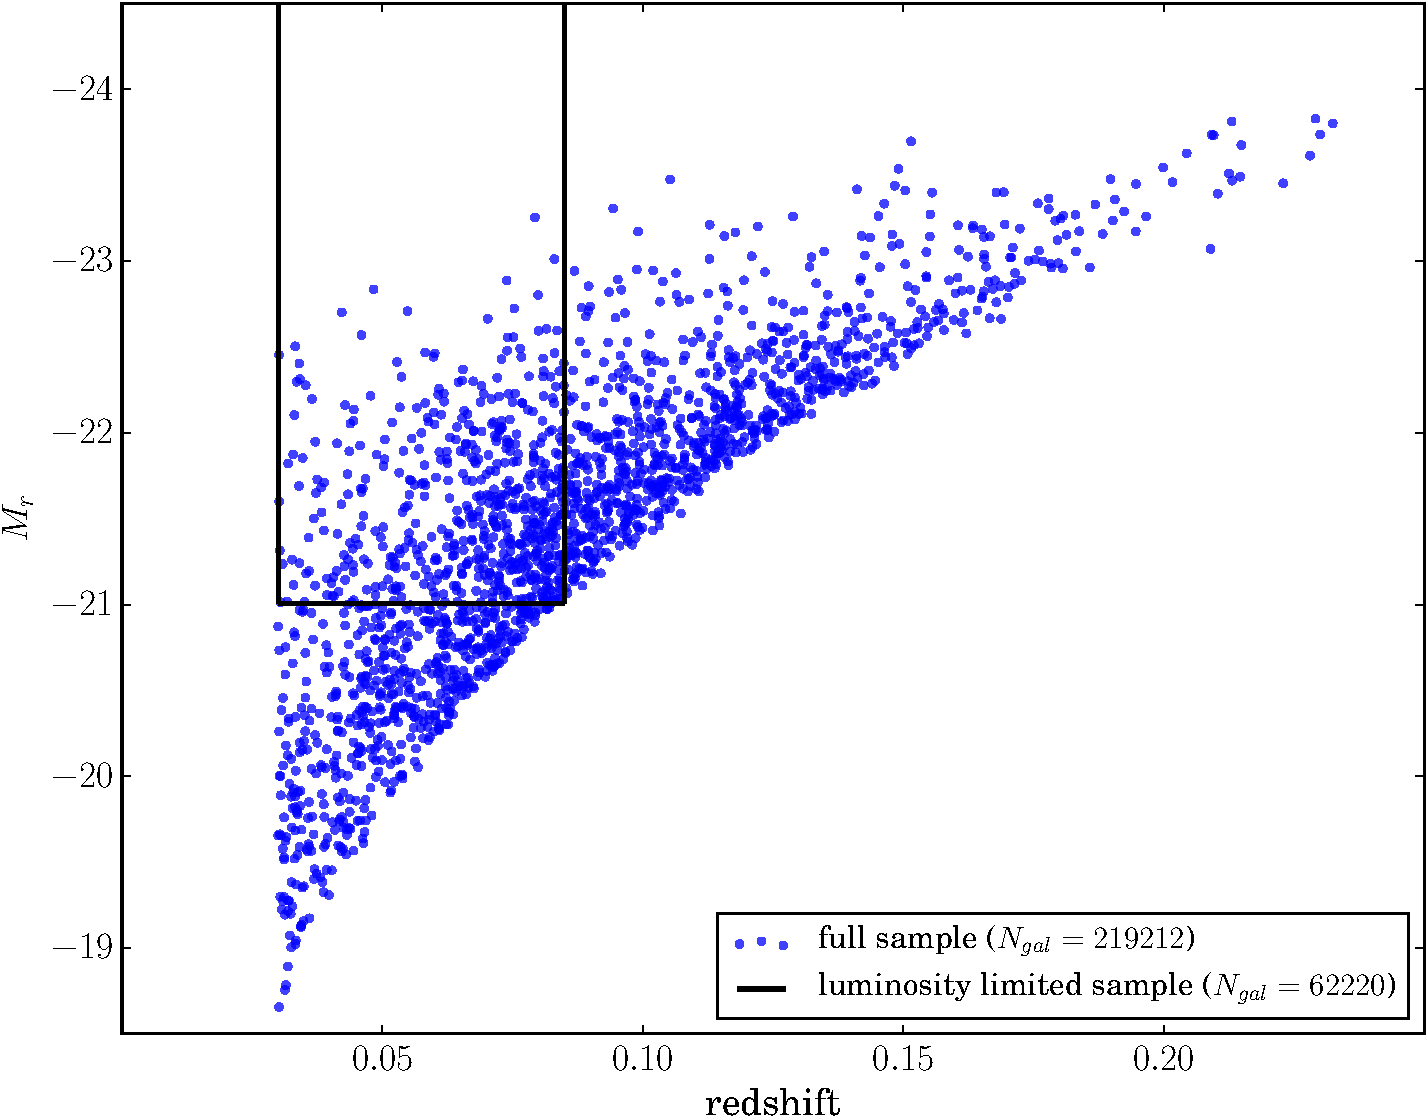
\includegraphics[width=0.5\textwidth]{Images/Data/volume_limited_sample.pdf}
    \caption{The $r$-band luminosity versus redshift distribution of our \textit{full sample} (blue points), with the region enclosing our $0.03<z<0.085$, $M_r  = -21.01$ \textit{luminosity-limited sample} indicated by black lines. Only a random selection of 2000 points are plotted for clarity.
		\label{fig:vl_sample}}
\end{figure}

In terms of stellar mass, the \textit{luminosity limited sample} is incomplete for the reddest galaxies at $\log (M/M_{\odot}) < 10.6$. Where necessary we therefore consider a \textit{stellar-mass-limited sample} of 41,801 galaxies, formed by applying a limit of $\log (M/M_{\odot}) \geq 10.6$ to the \textit{luminosity-limited sample}.

%------------------------------------------------------------------------------------

\subsection{Quantifying morphology with Galaxy Zoo}
\label{sec:gz_morphologies}

In GZ2, morphological information for each galaxy was obtained by asking participants to answer a series of questions (see figure 1 in W13) \rh{*actually put the tree here?}.  Typically, each image was viewed by $\ga 40$ people.  The result for each question is thus represented by the `vote fraction`, $p$ assigned to each possible answer. For any given answer, the sum of the $p$-values for all possible answers adds up to 1. Considering the 1st question as an example, if a galaxy was classified by 40 people, and 30 of those people said that the galaxy had features and the other 10 said that it was smooth, the corresponding $p$-values would be $p_{features}=0.75$ and $p_{smooth}=0.25$.  In order to reduce the influence of unreliable classifiers, \citet{Willett_13} weighted individual volunteers with respect to their agreement with the others.  Throughout this paper we refer to these weighted vote fractions as the `raw' quantities. However, before using these GZ2 vote fractions to study the galaxy population, we must first consider the issue of classification bias, as we shall in section \ref{sec:biases}.

Traditional morphologies assign each galaxy to a specific class, usually determined by one, or occasionally a few, experts. In contrast, Galaxy Zoo provides a large number of independent classifications for each galaxy.  This allows us to consider both the inherent `fuzziness' and observational uncertainties of galaxy morphology, and hence control the compromise between sample contamination and completeness.

There are two principal ways in which galaxy morphologies can be quantified using Galaxy Zoo vote fractions. The first is to consider averages of the vote fractions over specific samples or bins divided by some other property.  These average vote fractions can then be used to study variations in the morphological content of the galaxy population.  Individual galaxies are not given specific classifications.  There is no population of `unclassified', and hence ignored, galaxies.  This approach has been taken by \citet{Bamford_09}, \citet{Casteels_13}, \citet{Willett_15}, and various other studies. With this method, the vote fractions of all galaxies can be considered together; even galaxies with a small (but non-zero) vote fraction for a given property count towards the statistics. Effectively, this approach considers the vote fractions to estimate the probability of a galaxy belonging to a particular class.

The second approach is to divide the galaxy sample in to different morphological categories, either by applying a threshold on the vote fractions, or choosing the class with the largest vote fraction. Such methods have been used by \citet{Land_08}, \citet{Skibba_09}, and many more.  One advantage of this approach is that galaxies are assigned to definite classes with the threshold tuned to ensure a desired level of classification certainty.  However, a set of `uncertain' or `unclassified' galaxies may remain.  In some analyses these will require special attention.

These different approaches are also relevant for how questions at different levels in the tree are combined.  For example, participants are only asked if they can see spiral arms when they have already answered that they can see features in the galaxy and that the galaxy is not an edge-on disc.  The vote fraction for spiral arms therefore represents the conditional probability of spiral arms \emph{given that} features are discernible \emph{and} that the galaxy is not edge-on. When considering whether a galaxy displays spiral arms, one should account for the answers to these previous questions in the tree.  One can treat vote fractions as probabilities, multiplying them to obtain a `probability' that a galaxy displays any features, is not edge-on and possesses spiral arms.  Alternatively, one may first select galaxies that display features and are not edge-on and possess spiral arms, by applying some thresholds to the vote fractions for each question in turn. (See \citealt{Casteels_13} for a more thorough discussion of these issues.)

The primary morphological feature we will focus on in this paper is the apparent number of spiral arms displayed by a galaxy.  As we will see, some of the classes for this feature contain a relatively low fraction of the total spiral population.  In addition, the vote fractions for the preferred answer are often fairly low, with votes distributed over several answers.  In such cases, averaging the vote fractions over the full sample does not work particularly well, as noise from more common galaxy classes overwhelms the subtle signal from rarer classes.  In this paper we therefore prefer to assign galaxies to morphological samples by applying a threshold or taking the answer with the largest vote fraction.

%------------------------------------------------------------------------------------
%%%%%%%%%%%%%%%%%%%%%%%%%%%%%%%%%%%%%%%%%%%%%%%%%%%%%%%%%%%%%%%%%%%%%%%%%%%%%%%%%%%%%
%------------------------------------------------------------------------------------
\section{Correcting for redshift-dependent classification bias}
\label{sec:redshift_bias}
%------------------------------------------------------------------------------------
\subsection{Biases in the Galaxy Zoo sample}
\label{sec:biases}
Without any evolution in the population of galaxies, the `true' distribution of morphologies does not change. However, the apparent brightness and size of galaxies can change depending on the distance at which it is viewed \citep{Bamford_09}. The GZ2 sample includes SDSS galaxies and only includes galaxies up to a redshift of $\sim 0.25$, which is shallow enough to justify that there is no evolution in the true galaxy morphologies in our sample (W13). However, the sample is still susceptible to \textit{classification bias}, due to the effect of how the images are presented in Galaxy Zoo. Due to their distance, galaxies at high redshift appear fainter in the SDSS images than galaxies at lower redshift, and therefore have lower signal-to noise. This means that more detailed features may be more difficult to distinguish in galaxies at higher redshift. It should also be noted that such biases are not exclusive to Galaxy Zoo- difficulty in observing faint features in lower signal-to-noise galaxies is an inherent property of any visual galaxy classifications. The advantage of using Galaxy Zoo classifications is that it gives us a statistical method of looking at galaxy morphologies- as each of the galaxies in the full galaxy sample has been visually classified by a number of independent observers, we can model how the apparent presence of features evolves with redshift, and correct this bias accordingly.

The effect of classification bias is an important property that must be corrected for if we want to compare morphologies using either of the two techniques discussed in section \ref{sec:gz_morphologies}. Sample incompleteness and sample contamination are defects that arise in a sample where an inherent redshift bias affects the classifications.  Sample incompleteness affects the `harder to see' features- the number of galaxies classified as having a particular feature would decrease with redshift in this case, leaving us with poor number statistics for such galaxies.  Sample contamination is the converse effect that appears in the 'easier to see' features.  In this case, the samples we define using the GZ classifications also include mis-classified galaxies that should have actually been included in one of the `harder to see' categories, meaning that any differences observed by comparing different features may be negated. 

The effect of redshift bias is shown in Fig.~\ref{fig:vote_histograms}a, where a high and low-redshift \textit{luminosity-limited sample} are compared. As this is a \textit{luminosity-limited sample}, the overall galaxy population should not change with redshift. However, a greater fraction of the galaxies have lower values for $p_{features}$ in the higher redshift sample, as classifiers have greater difficulty picking out features in the higher redshift, lower signal-to-noise images. If we wished to compare a sample of galaxies with `features' against one that is `smooth', then the number of galaxies with `features' would be incomplete, as a greater fraction of the galaxies would be classified as `smooth' at higher redshift (making the sample of `smooth' galaxies contaminated).

\begin{figure}
		\centering

        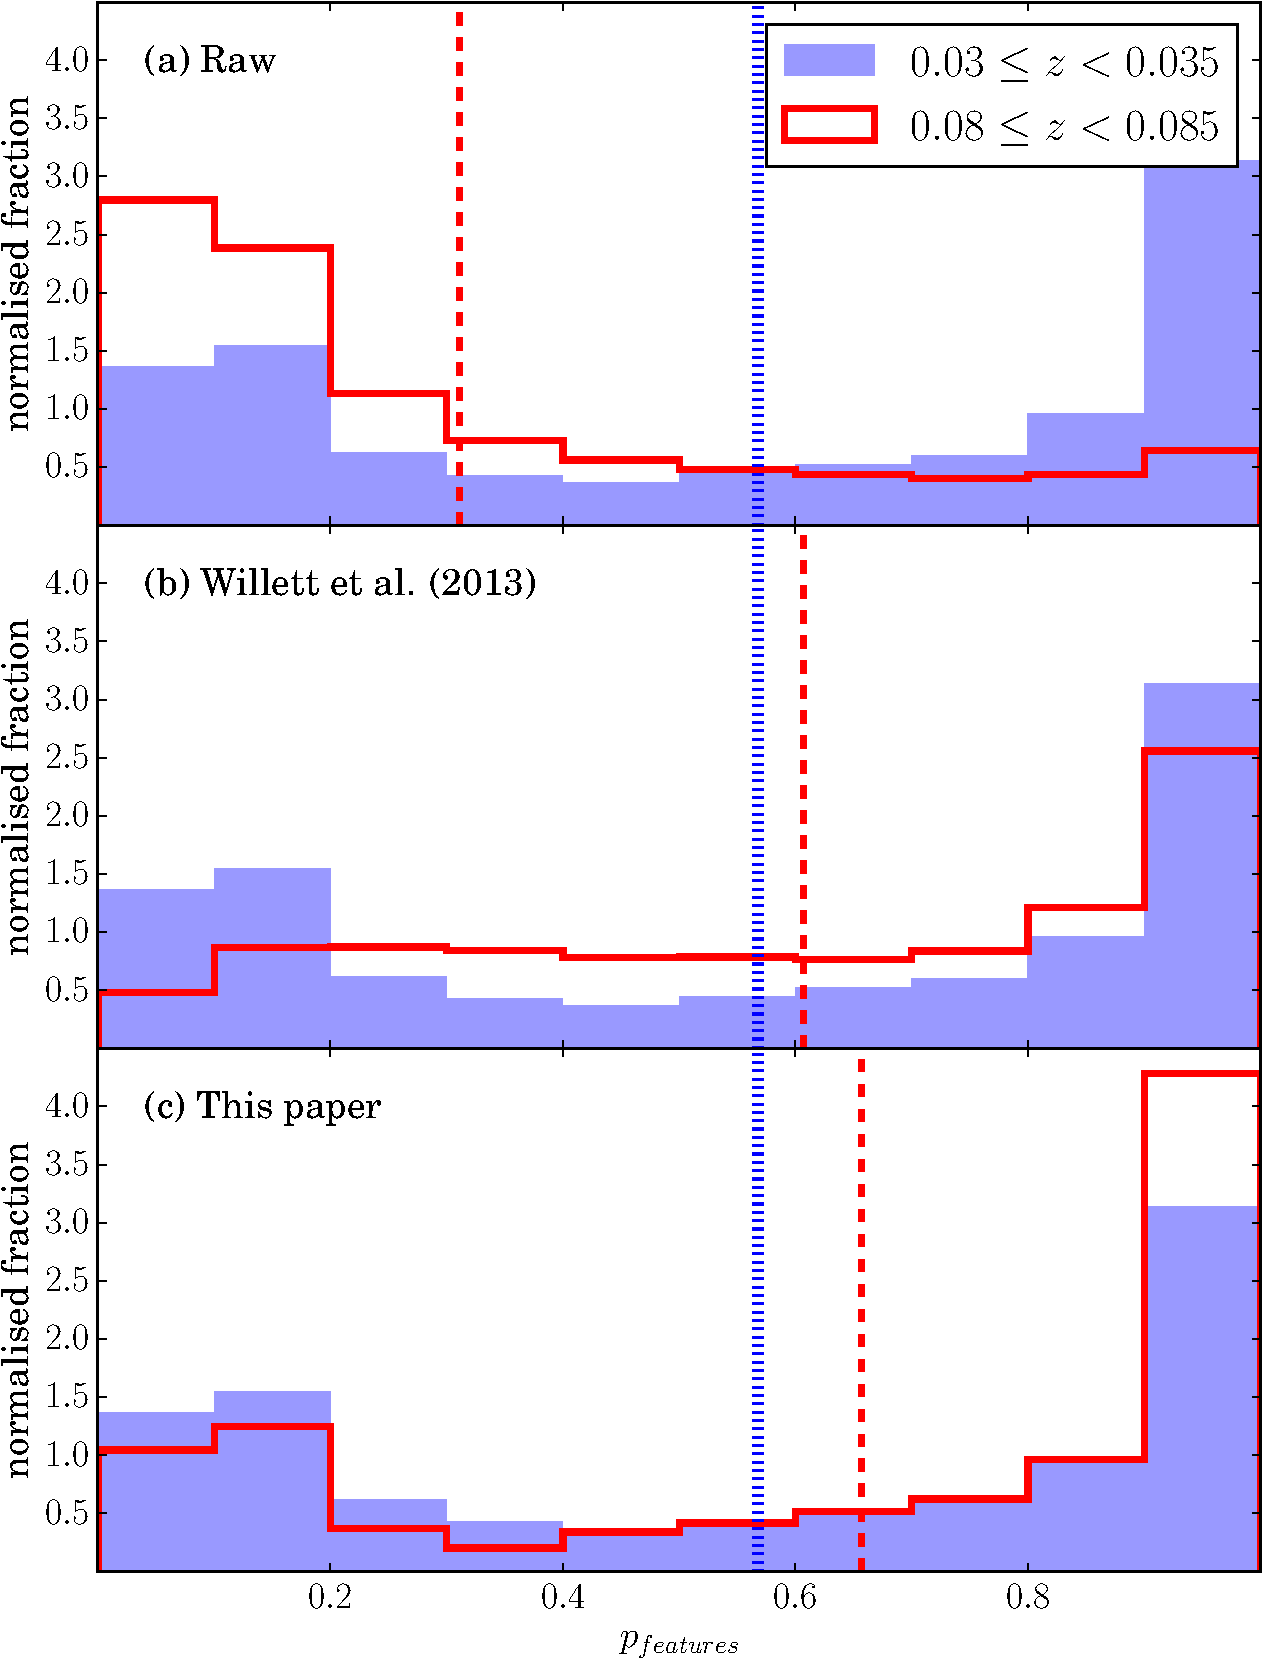
\includegraphics[width=0.5\textwidth]{Images/Bias/Biases/comparison_histogram.pdf}

        \caption{Histograms of vote distributions for the question of whether galaxies are `smooth' or contain `features' in GZ2. The filled blue histogram shows a low redshift sample and the red line indicates a high redshift sample. Both samples are from the \textit{luminosity-limited sample}. The dotted blue line indicates the mean $p_{features}$ value from the low-redshift sample and dashed red line shows the same value for the higher-redshift sample.}

        \label{fig:vote_histograms}

\end{figure}

%------------------------------------------------------------------------------------
\subsection{Previous attempt to correct for redshift bias}
\label{sec:previous_method}

The previous debiasing procedure applied to both GZ1 and GZ2 has focused on adjusting the vote fractions of the galaxy samples by fixing the mean vote fractions as a function of redshift. The method was first proposed in \cite{Bamford_09}, and updated for GZ2 in W13. The method successfully adjusts the mean vote fraction for questions with two dominant answers, as can be seen from the vertical lines in figure \ref{fig:vote_histograms}b- the red dashed line of the high-redshift sample is much closer to the blue vertical line from the low-redshift sample than in the raw vote distributions (Fig.~\ref{fig:vote_histograms}a).

However, this technique has two limitations that make it unsuitable if we want to divide a galaxy sample in to different morphology subsets.  The first issue is that adjustment of the mean vote fraction does not necessarily lead to correct adjustment of individual vote fractions, an effect that can be seen in Fig.~\ref{fig:vote_histograms}b.  Although the mean fractions for the high-redshift sample have been correctly adjusted to approximately match the low-redshift sample, the overall distributions are not necessarily correctly adjusted. Although the mean values match, we see that there is an excess of debiased votes in the middle of the distribution, and fewer votes for the tails of the distribution at $p \approx 0$ and $p \approx 1$. This effect is important if we wish to divide our sample into different subsets by morphological type- as the shape of the histograms is not consistent with redshift, the fraction of galaxies with $p_{features}$ greater than a given threshold can also vary with redshift.\rh{perhaps a quick figure to show that this is happening???}

As described in section \ref{sec:gz_morphologies}, GZ2 utilises multiple answered questions to obtain more detailed classifications of galaxies than GZ1. In cases where the votes are split between multiple categories, the debiasing method from W13 does not adjust all of the vote fractions correctly. To show this effect, we select a sample of `secure' spiral galaxies with $p_{\textrm{features}} \times p_{\textrm{not edge-on}} \times p_{\textrm{spiral}} > 0.5$, (with the $p$ value corresponding to the debiased values from W13), and plot the mean $p$-values with respect to redshift. A clear trend in $p$ with redshift is observed- the mean $p$ values increase with redshift for the 1 and 2 spiral arm answers, even after the W13 correction has been applied. For this question, the answers with more spiral arms (3,4 or more than 4 spiral arms) are the `harder to see' features meaning that there are fewer votes for these categories overall at higher redshift. The W13 debiasing method does not adequately adjust the votes with respect to redshift, so we require an alternative method of debiasing to ensure our galaxy samples are complete at all redshifts. We will now describe this new method in Sec.\ref{sec:new_method}.

\begin{figure}
		\centering

        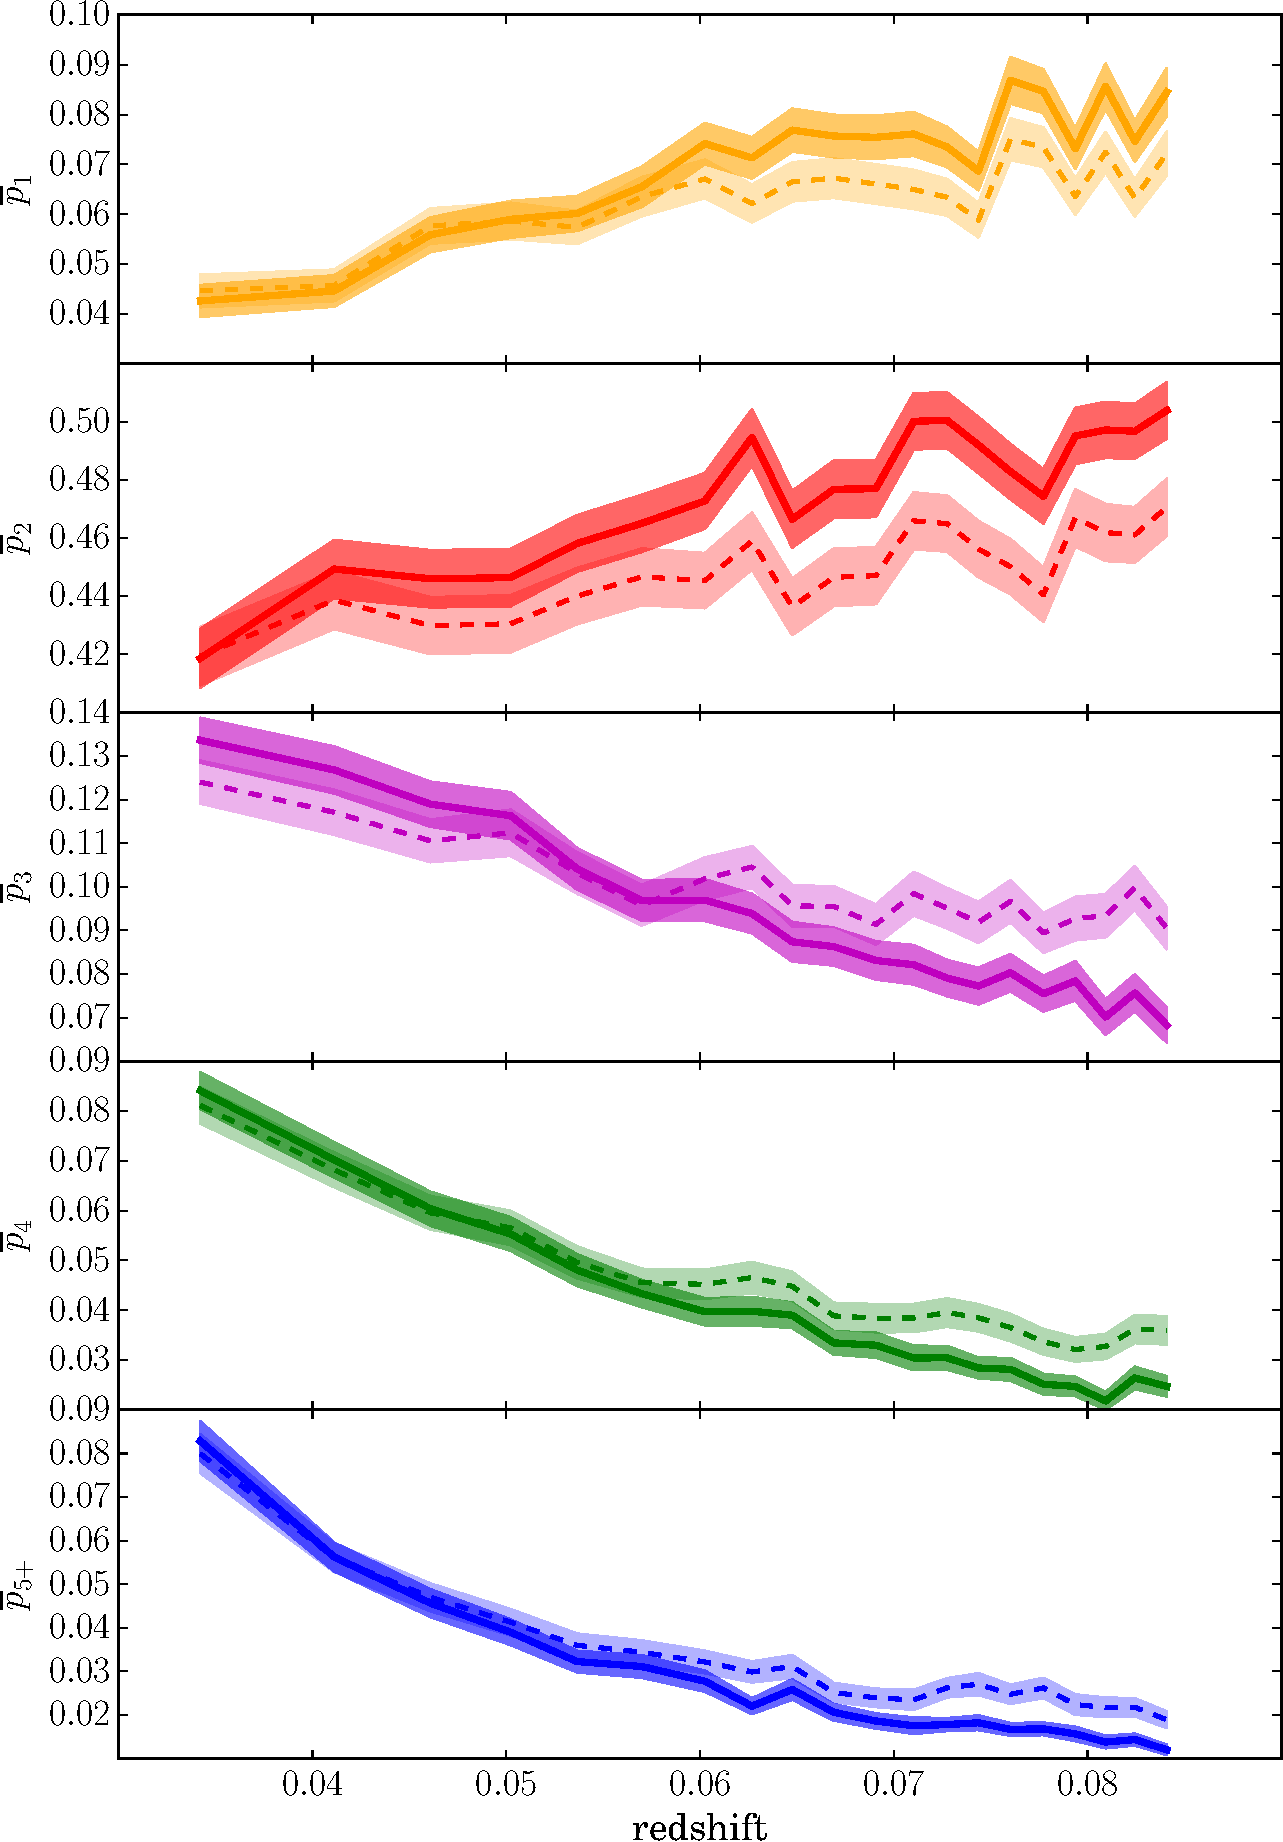
\includegraphics[width=0.5\textwidth]{Images/Bias/Biases/mean_arm_fractions.pdf}

        \caption{Mean value of $p$ for each of the arm number questions. The sample consists of galaxies from the \textit{luminosity-limited sample}, with $p_{features} \times p_{not \, edge-on} \times p_{spiral} > 0.5$, with $p$-values taken from the W13 debiased catalogue. The solid lines show the values obtained using the raw vote classifications, and the dashed lines indicate the corresponding values from the debiased values from W13. The shaded regions indicate the $1 \sigma$ error on the mean.}

        \label{fig:arm_bias}

\end{figure}

%------------------------------------------------------------------------------------
\subsection{A new method for removing redshift bias}
\label{sec:new_method}

With the limitations described in Sec.~\ref{sec:previous_method}, we attempt to construct a new method of debiasing the GZ2 data more effectively. This is of particular importance when looking at the question of spiral arm multiplicity. This is because for a volunteer to have answered the question regarding arm multiplicity, they must have answered a specific answer to three questions previously (that the galaxy has features, is not edge-on and does have spiral arms). Therefore, the number statistics for such galaxies can be very low. When considering a question with low number statistics, such as the spiral arm question, we prefer to use a thresholding technique, rather than using the weighted $p$-values (see Sec.~\ref{sec:gz_morphologies} for a descriptions of both methods). This is because rarer classes of objects will be affected by noise from the more dominant categories (in this case the 2-armed answer). We therefore prefer to divide our galaxy sample in to different sub-samples in order to directly compare them. However, if we wish to use a thresholding technique to achieve this, it is important that each of the questions `further up' the decision tree has already been debiased, so that all samples are complete with redshift.

Unlike the debiasing method in W13, our new method aims to make the vote distributions themselves as consistent as possible with redshift rather than purely aiming for consistency in the mean vote fraction values. As each galaxy is classified by 40 or more volunteers (W13), we have enough data to model the evolution of the vote distributions as a function of redshift. The theory behind this method is that different classifiers will have different levels of ability to pick out the most detailed features. Thus, as we consider samples at higher redshift, where images have lower signal-to noise, we expect the overall vote fraction trends to also evolve as some classifiers become less able to see the most detailed features. We aim to model this redshift bias by modelling the vote fraction distributions as a function of redshift, and correcting the higher redshift vote distributions to be as similar as possible to equivalent vote distributions at low redshift. 

To do this, we first define samples of galaxies with $p>0.5$ for each of the questions in turn. The entire galaxy sample is then binned in terms of the intrinsic galaxy properties of size and luminosity, and each of these bins is divided in to redshift slices. We then attempt to model the vote distributions for each of the bins with respect to redshift, matching their distributions to those at low redshift. This means that if a threshold is made, the fraction of galaxies with a given feature remains constant, and the sample is composed of the galaxies that are most likely to have that particular feature.It must also be noted that such a method could still be limited by number statistics at higher redshift. In the case that a rare feature's $p$ value drops to 0 at higher redshift, we can not `add-in' votes- it is only possible to debias the galaxies with $p>0$ which may change significantly with redshift in the rarest categories where the vote fractions are lowest.

%------------------------------------------------------------------------------------
\subsubsection{Sample selection for each question}
\label{sec:sample_selection_per_question}

As GZ2 morphologies are classified with a decision tree (see section \ref{sec:gz_morphologies}), not all of the questions were answered by each of the volunteers. Using the example of spiral arm number, for an individual classifier to have answered the question regarding arm number, they would also have needed to answer that the galaxy they saw had features, was not edge-on and had spiral arms. To avoid `noise' introduced by incorrectly classified galaxies, clean galaxy samples are defined with $p > 0.5$. For the first question, this corresponds to all of the galaxies, as each classifier answered that particular question for each galaxy. However, when questions further down the tree are considered, this is not the case. The equiavalent $p>0.5$ for the spiral arm question would only include the galaxies with $p_{\textrm{features}} \times p_{\textrm{not edge-on}} \times p_{\textrm{spiral}} > 0.5$. 

For each of the question in turn, we define a sample of galaxies with which we will apply the new debiasing procedure. For each of the questions, we define a sample of galaxies with which we model the bias with respect to redshift. We define these secure samples using a cut of $p>0.5$ (corresponding to $p_{\textrm{features}} \times p_{\textrm{not edge-on}} \times p_{\textrm{spiral}} > 0.5$ for the spiral arm question for example). A further cut of $N \geq 5$ (where $N$ is the number of classifications) is also imposed to ensure that each galaxy has been looked at by a significant number of people to reduce the effects of noise. In this case, the $p$ values are our debiased vote values, to ensure each sample is as complete as possible (see Sec.~\ref{sec:biases}) as we look at each question.
%------------------------------------------------------------------------------------
\subsubsection{Binning the data}
\label{sec:binning}

It is expected that bin properties depend on intrinsic galaxy properties, in particular size and luminosity. For example, larger, brighter galaxies may be easier to classify over a wider range of redshift. Conversely, fainter galaxies may show stronger features, as they should be composed of a greater fraction of spiral galaxies \rh{reference????} than the larger, brighter galaxies. To account for this, we voronoi tesselate the data in terms of $M_r$ and $\log(R_{50})$ for each answer in turn using the \texttt{voronoi\_2d\_binning} package from \cite{Cappellari_03}, meaning that each of the bins should contain an aproximately equal number of galaxies. When voronoi tesselating the data for each of the answers, only the galaxies with $p>0$ are included, meaning that the `signal' of galaxies is evened out over all of the voronoi bins. We aim to have $\sim 30$ voronoi bins for each of the questions, so the bin signal for each of the voronoi bins is given as $N_{gal}/30$, where $N_{gal}$ is the number of galaxies with $p>0$. An example of a voronoi tesselation is shown in Fig.~\ref{fig:voronoi_bins}. 

\begin{figure}
		\centering

        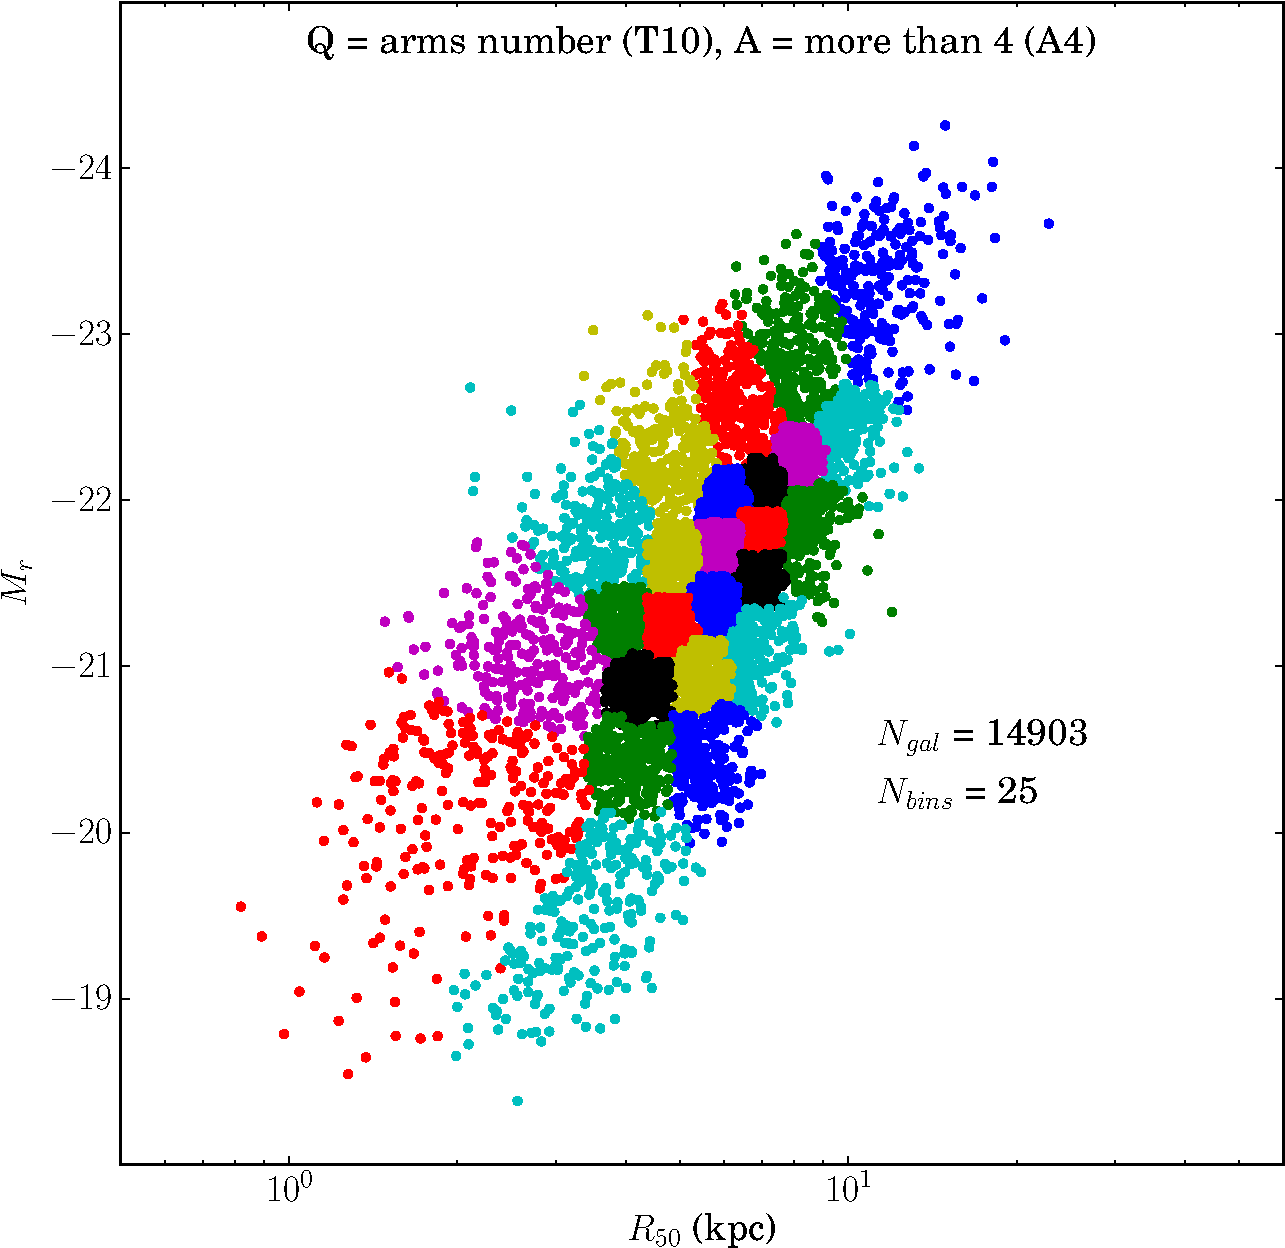
\includegraphics[width=0.5\textwidth]{Images/Bias/Debiasing/voronoi_bins.pdf}

        \caption{Distribution of the voronoi bins in terms of $R_{50}$ and $M_r$ for the spiral arm number question and the more than 4 spiral arms answer. Each of the voronoi bins is further divided in to redshift bins, each with $\geq 100$ galaxies.}

        \label{fig:voronoi_bins}

\end{figure}

After voronoi binning the data in terms of their intrinsic properties of size and brightness, we further divide the sample in to redshift bins, to allow us to look in to how the vote distributions change with redshift. To ensure that there is a good signal in each of the redshift bins, we divide each of the voronoi bins in to redshift bins containing $\geq 100$ galaxies each. This binned data is used for the debiasing methods described in section \ref{sec:debiasing}.

%------------------------------------------------------------------------------------
\subsubsection{Modelling redshift bias}
\label{sec:debiasing}

For each of the possible responses to each question, a method is applied to correct for the redshift bias in the sample. The first stage is to select a sample as described in section \ref{sec:sample_selection_per_question} as a reference, and to bin the data using the method described in section \ref{sec:binning}. As described in section \ref{sec:new_method}, we aim to make the vote distributions for each answer consistent with redshift. The two methods that we employ to achieve this are described below. 

The first method we utilise remove redshift bias simply matches the shapes of the histograms on a `bin-by-bin' basis. The vote fractions for the given answer are ranked from lowest $p$-value to highest $p$-value, and a cumulative histogram is plotted. The cumulative distribution for the lowest redshift sample in a given voronoi bin is used as a reference for how the shape of the histogram would look if it were viewed at low redshift. An example of this method is shown in Fig.~\ref{fig:histogram_matching}, in which the `features or disk' answer to the `smooth or features' question is considered. For each of the higher redshift samples in that same voronoi bin, the ranked votes are matched to those at lower redshift. This means that applying a threshold gives the same fraction of galaxies above that given threshold in both the high and low redshift bins, with the galaxies most likely to have a given feature making up the population of galaxies above that threshold. 

\begin{figure}
		\centering

        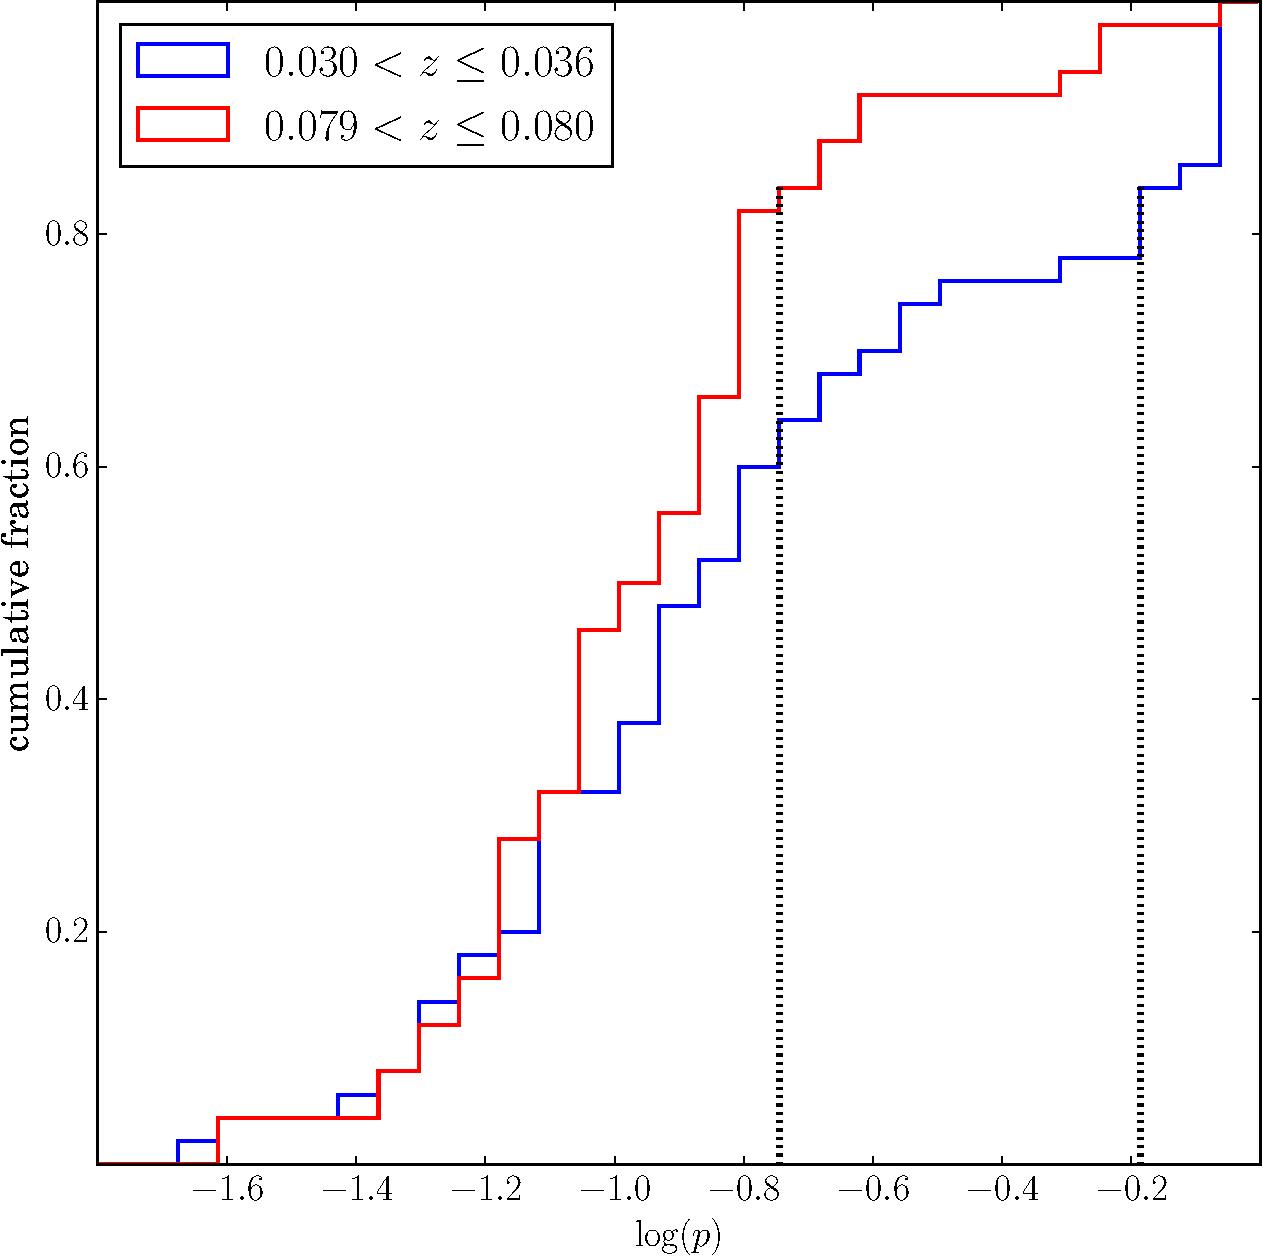
\includegraphics[width=0.5\textwidth]{Images/Bias/Debiasing/histogram_matching.pdf}

        \caption{An example of vote distributions for an example voronoi bin for the `features or disk' answer to the `smooth or features' question. Each of the galaxies in the high-redshift bin (red line) is matched to its closest equivalent low-redshift galaxy (blue line) in terms of cumulative fraction. The dashed lines indicate the `matched' values for an example galaxy with $\log(p) \approx 0.8$, and an equivalent low-redshift value of $\log(p) \approx 0.2$(corresponding to $p_{raw}=0.18$ and $p_{debiased}=0.65$).}

        \label{fig:histogram_matching}

\end{figure}

The main advantage of this method is that any vote distribution can be modelled in this way, irrespective of the overall shape. However, a weakness of the above method is that noise can be introduced due to the discretisation of the data. This can cause issues when the number statistics are low in questions where the sample size is severely reduced because of the number of questions that have come before it (see Sec.~\ref{sec:sample_selection_per_question}), which means that the bins have to span a wide redshift range to achieve a `good' signal of 50 galaxies per bin. One potential solution would be to bin the data more finely. However, there is no `ideal' solution to this problem- fewer galaxies in each bin would mean that the redshift range that each bin occupies would be less, but the overall noise in terms of the range of galaxy morphologies within each bin would increase. 

To attempt to remove the discrete nature of the correction in the `bin-by-bin' method, an alternative approach is proposed that attempts to model vote distributions with functions. For each of the redshift bins, we plot a cumulative histogram of $\log(p)$ against cumulative fraction, as indicated in the solid lines of Fig.~\ref{fig:function_fit}. Each of the cumulative histograms is then modelled with an exponential power function of the following form:

\begin{equation}
f(p) = e^{kp^{c}}
\end{equation}

where $k$ and $c$ parameterise the shape of each of the curves. Best-fit $k$ and $c$ values are found for each of the bins using the \texttt{scipy.optimize.minimize} package (\rh{cite?}), indicated by the dashed lines in Fig.~\ref{fig:function_fit}. When fitting the data, the data is sampled evenly in $\log(p)$ to avoid the fit being weighted to the most steep parts of the curves. 

After finding $k$ and $c$ for each of the bins, we attempt to quantify how these parameters change with respect to $M_r$, $\log(R_{50})$ and $z$. Firstly, we apply a $2\sigma$ clipping to $k$ and $c$ to remove any fits that has extreme $k$ or $c$ values have been found. The data is then fitted using a function of the following form:

\begin{equation}
\begin{split}
A_{fit}(M_r,R_{50},z) = & A_0 + A_M(f_M(-M_r)) +\\
						& A_R(f_R(\log({R_{50}}))) + A_z(f_z(z))
\end{split}
\end{equation}

where $A$ corresponds to either $k$ or $c$ and $f_M$, $f_R$ and $f_z$ are functions that can be either logarithmic ($\log(x)$), linear ($x$) or exponential ($e^x$) (where x is either $-M_r$, $\log(R_{50})$ or $z$). The values $A_0$, $A_M$, $A_R$ and $A_z$ are constants that parameterise the shape of the fit with respect to each of the terms. When fitting the data, $M_r$, $\log{R_{50}}$ and $z$ correspond to their respective mean values for each of the bins, which has an associated fit $k$ and $c$ value. The best combination of functions is chosen by calculating $A_0$, $A_M$, $A_R$ and $A_z$ for each combination of $f_M$, $f_R$ and $f_z$ using the \texttt{scipy.optimize.curve\_fit} package, and selecting the function that has the lowest square residual to find $k_{fit}$ and $c_{fit}$ continuous functions. We then clip any values with a $>2\sigma$ residual and re-fit the data to find a final functional form for $k$ and $c$ with respect to $M_r$, $R_{50}$ and $z$. Some $k_{fit}$ and $c_{fit}$ values at the $M_r$, $R_{50}$ and $z$ values of the bins for the spiral arm number question are shown by the dotted lines of Fig.~\ref{fig:function_fit}.

\rh{*Do we need some kind of plot to show how k and c have been fitted here?}

We also apply limits to $k$ and $c$ to avoid unphysical fits at extreme values of $M_R$, $R_{50}$ and $z$. We do this by calculating the the standard deviation of $k$ and $c$ (from the $2\sigma$ clipped values). The range of $k$ and $c$ is then set by the upper and lower limits of all of the fit $k$ and $c$ values.

After finding a functional form for $k$ and $c$ with respect to $M_r$, $\log(R_{50})$ and $z$, each of the galaxies in the sample is debiased to find equivalent values at low redshift. To do this for an individual galaxy, the shape of its cumulative histogram is estimated using $k_{fit}(M_r,R_{50},z)$ and $c_{fit}(M_r,R_{50},z)$, where $M_r$,$R_{50}$ and $z$ are the properties for that particular galaxy. The equivalent function at $z=0.03$ (the low redshift limit of our \textit{luminosity-limited sample} is also found for a galaxy with the same size and luminosity, using $k_{fit}(M_r,R_{50},0.03)$ and $c_{fit}(M_r,R_{50},0.03)$. The corresponding $p$-value \emph{for a given cumulative fraction} is read off from the low redshift distribution in a similar way as in the bin-by-bin method, but this time using the fitted curves rather than the raw histograms. This is repeated for each of the galaxies in the sample to generate our debiased values for the answer being considered.

\begin{figure*}
		\centering

        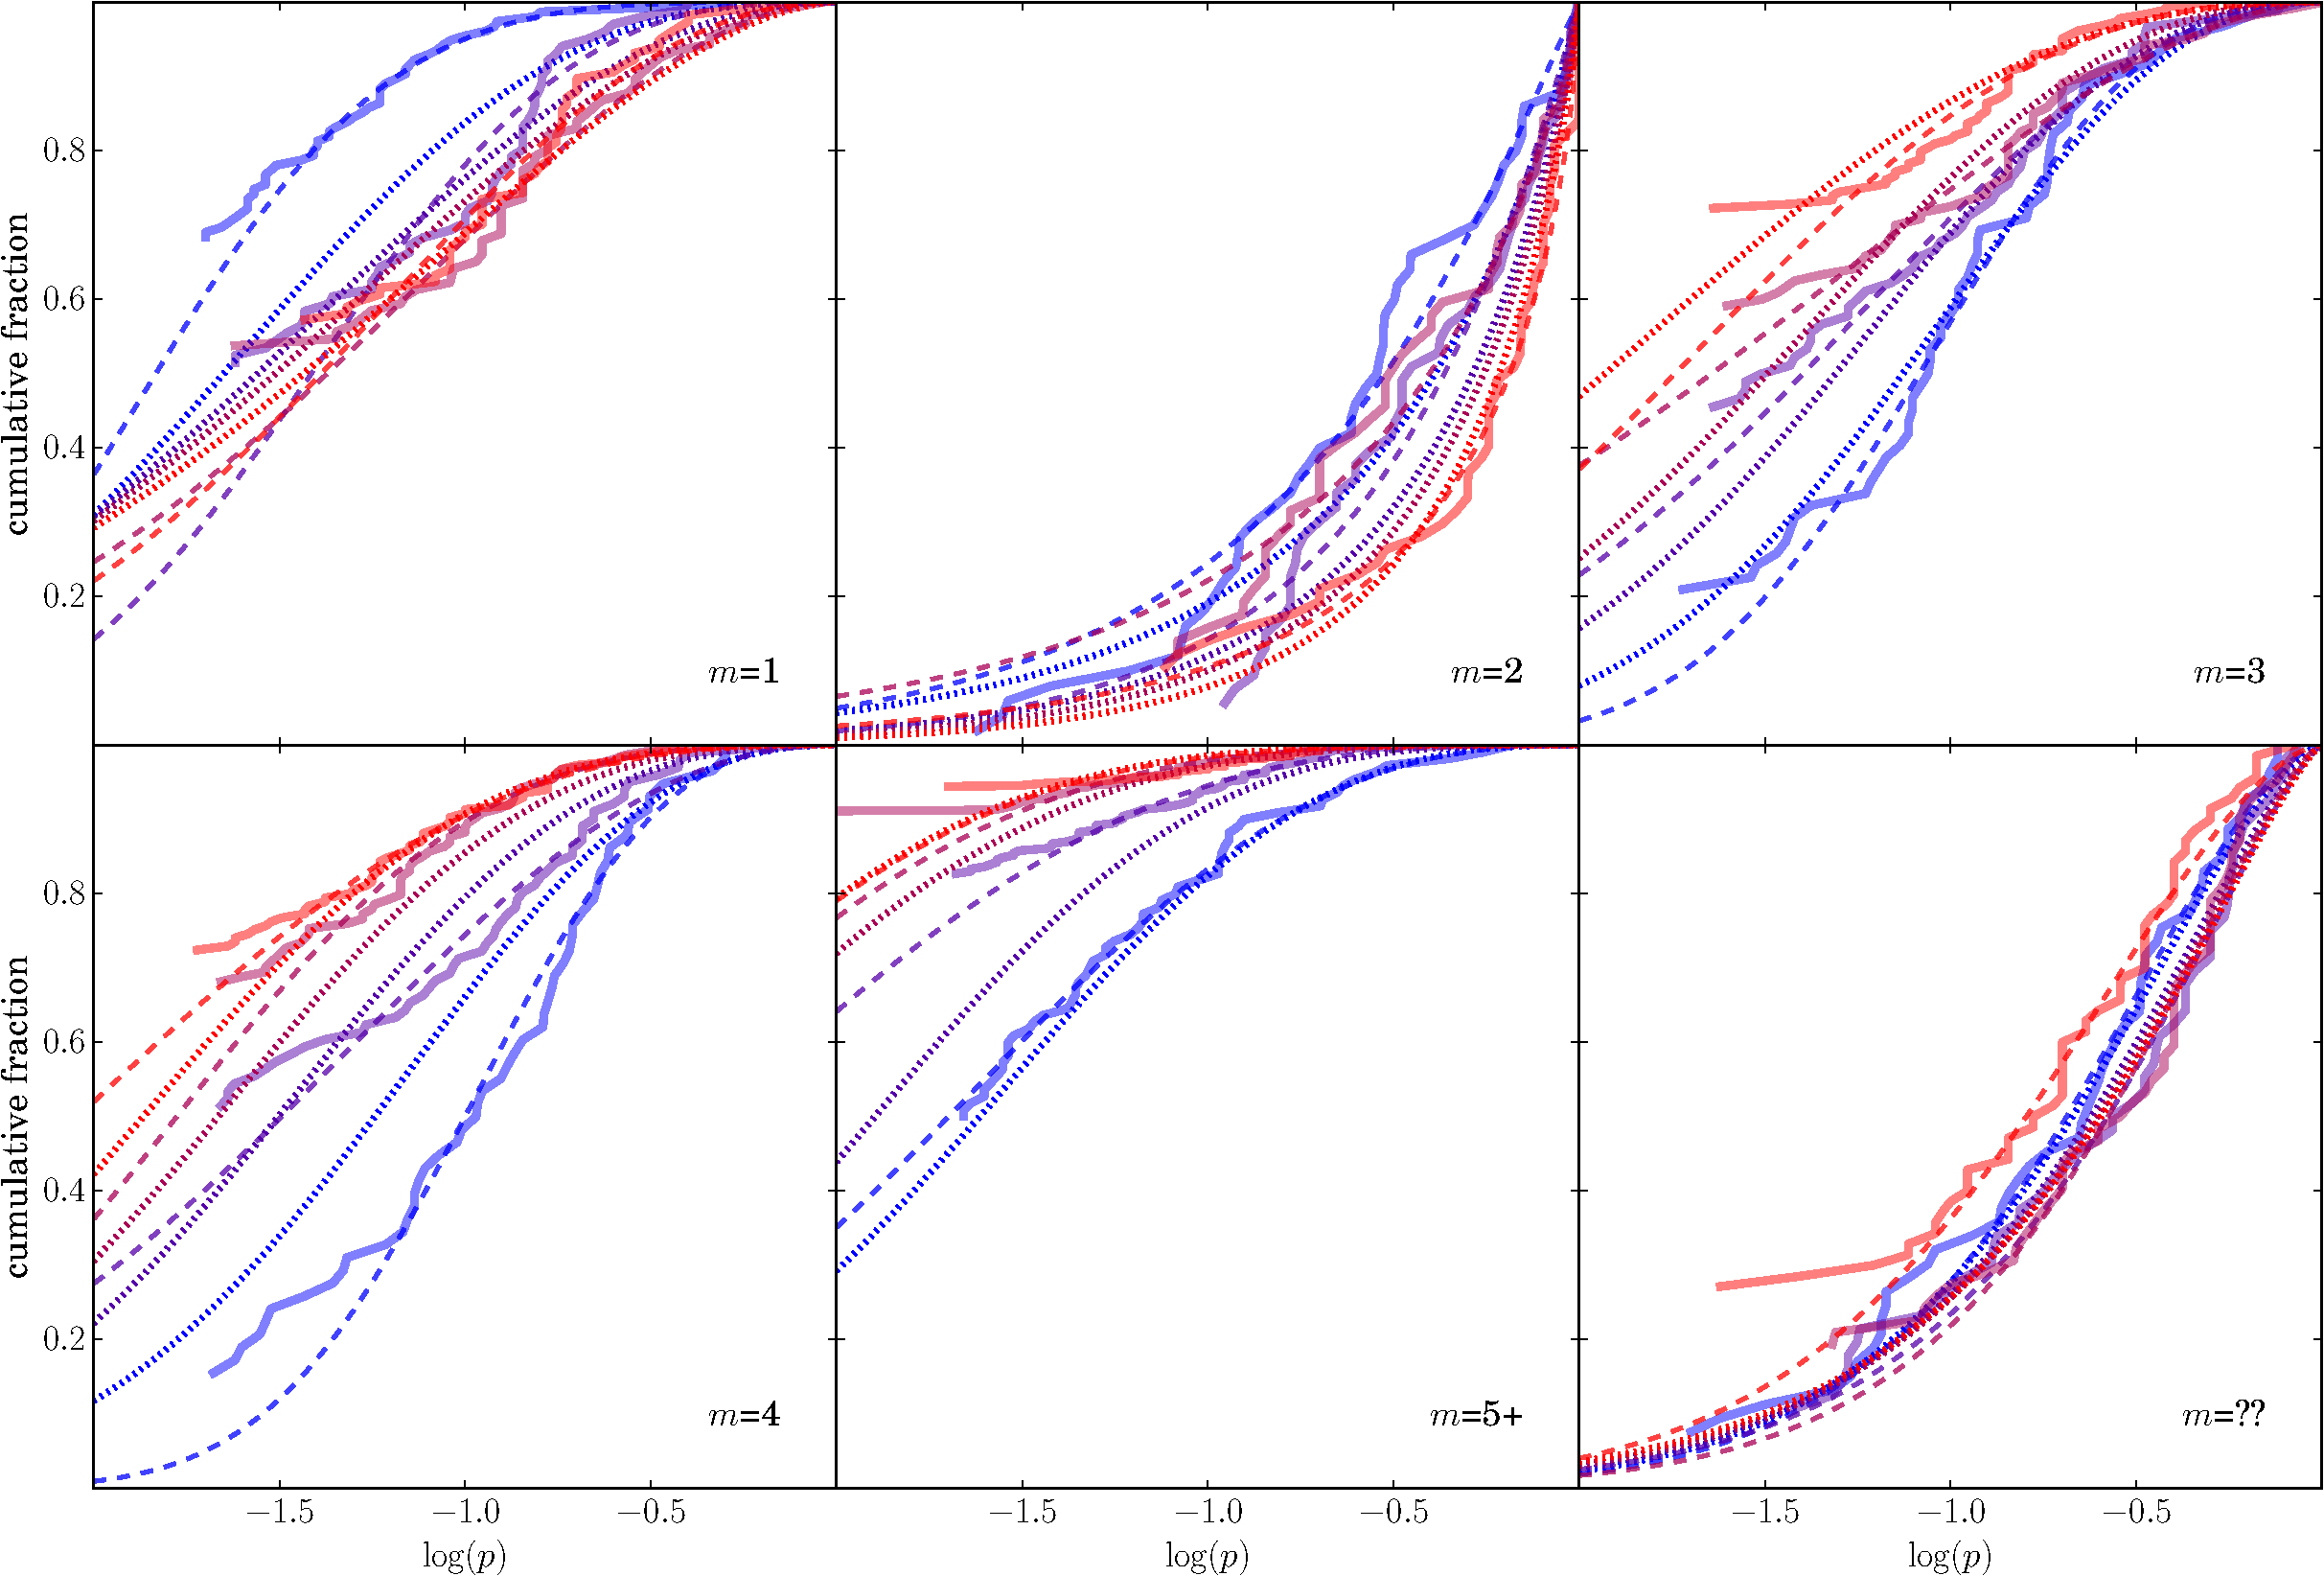
\includegraphics[width=1\textwidth]{Images/Bias/Debiasing/vbin_fit.pdf}

        \caption{An example of a single voronoi bin fit for the `arm number' question. The red line indicates the highest redshift bin, and the blue line indicates the lowest redshift bin. The solid lines indicate the raw $p$ histograms, and the dashed lines show the best fit function to each of the corresponding histograms. The dotted lines show the corresponding approximation from the continous fit to the $k$ and $c$ values.}

        \label{fig:function_fit}

\end{figure*}

As mentioned previously, function fitting does not suffer from the defects introduced by the discretisation of the data. However, it does introduce its own biases, as an assumption is made that the cumulative histograms can all be well-fit by a continuous function. However, this may not always be the case, so we must consider which of the above methods does the best overall job of removing redshift bias. To do this, we use the \textit{luminosity-limited sample} defined in section \ref{sec:sample}, as it should not be subject to any evolution in the overall galaxy population (see Sec.~\ref{sec:sample}). We take a low-redshift slice of this sample in the range $0.03 < z \leq 0.035$ as a reference, which should have minimal redshift bias. We then compare the raw vote fractions from the low-redshift sample with those of the total \textit{luminosity-limited sample} from both of our debiasing methods. To do this, we divide the \textit{luminosity-limited sample} in to 10 redshift bins, each containing the same number of galaxies. For each of these redshift bins, the residual is calculated by dividing the sample in to 10 bins of $p$ (ranging from 0 to 1 in steps of 0.1) and calculate the fraction of galaxies in each of these $p$ bins. The square residual is then calculated with respect to the equivalently binned data in the low-redshift reference sample. We take the sum of all of the square residuals to calculate a total square residual of the entire \textit{luminosity-limited sample}. The method that is deemed to have done the best job at debiasing the data is taken as the one with the lowest overall square residual, and the debiased values from that method are selected as the debiased values for that particular question. 

%------------------------------------------------------------------------------------

\subsubsection{Results from the new debiasing method}
\label{sec:debiasing_results}

As described in Sec.~\ref{sec:new_method}, our new method aims to keep the number of galaxies above a given threshold constant with redshift, rather than simply correcting the mean overall $p$-values with redshift. To test how successful the new debiasing method is at defining populations of galaxies above a given threshold with redshift, we plot the fraction of galaxies with $p>0.5$ for each of the questions in Fig.~\ref{fig:all_thresholds}. We plot only the \textit{luminosity-limited sample}, which should be free of any selection biases, meaning the overall galaxy distribution should not change with redshift. It can be seen that in most cases, the new debiasing method does keep the fraction of the population with $p>0.5$ constant with redshift, as expected. This effect is most evident when looking at the `spiral or no spiral' question, in the top right-hand side of Fig.~\ref{fig:all_thresholds}. It can be seen that the original debiasing method does not adequately remove redshift bias, with fewer galaxies exhibiting spiral structure at higher redshift. However, our  method does keep this fraction constant with redshift, which means our spiral sample will be complete if we wish to use a thresholding technique to separate galaxies in to samples of galaxies with spiral structure and galaxies which do not. However, it appears that for the given cut of $p>0.5$, there are cases where the W13 debiasing method looks peferable, for example in the `smooth or features' question. However, it must also be noted that this plot only shows the redshift trend for a single threshold in $p$, and may not be the case for different $p$ thresholds.

\begin{figure*}
		\centering

        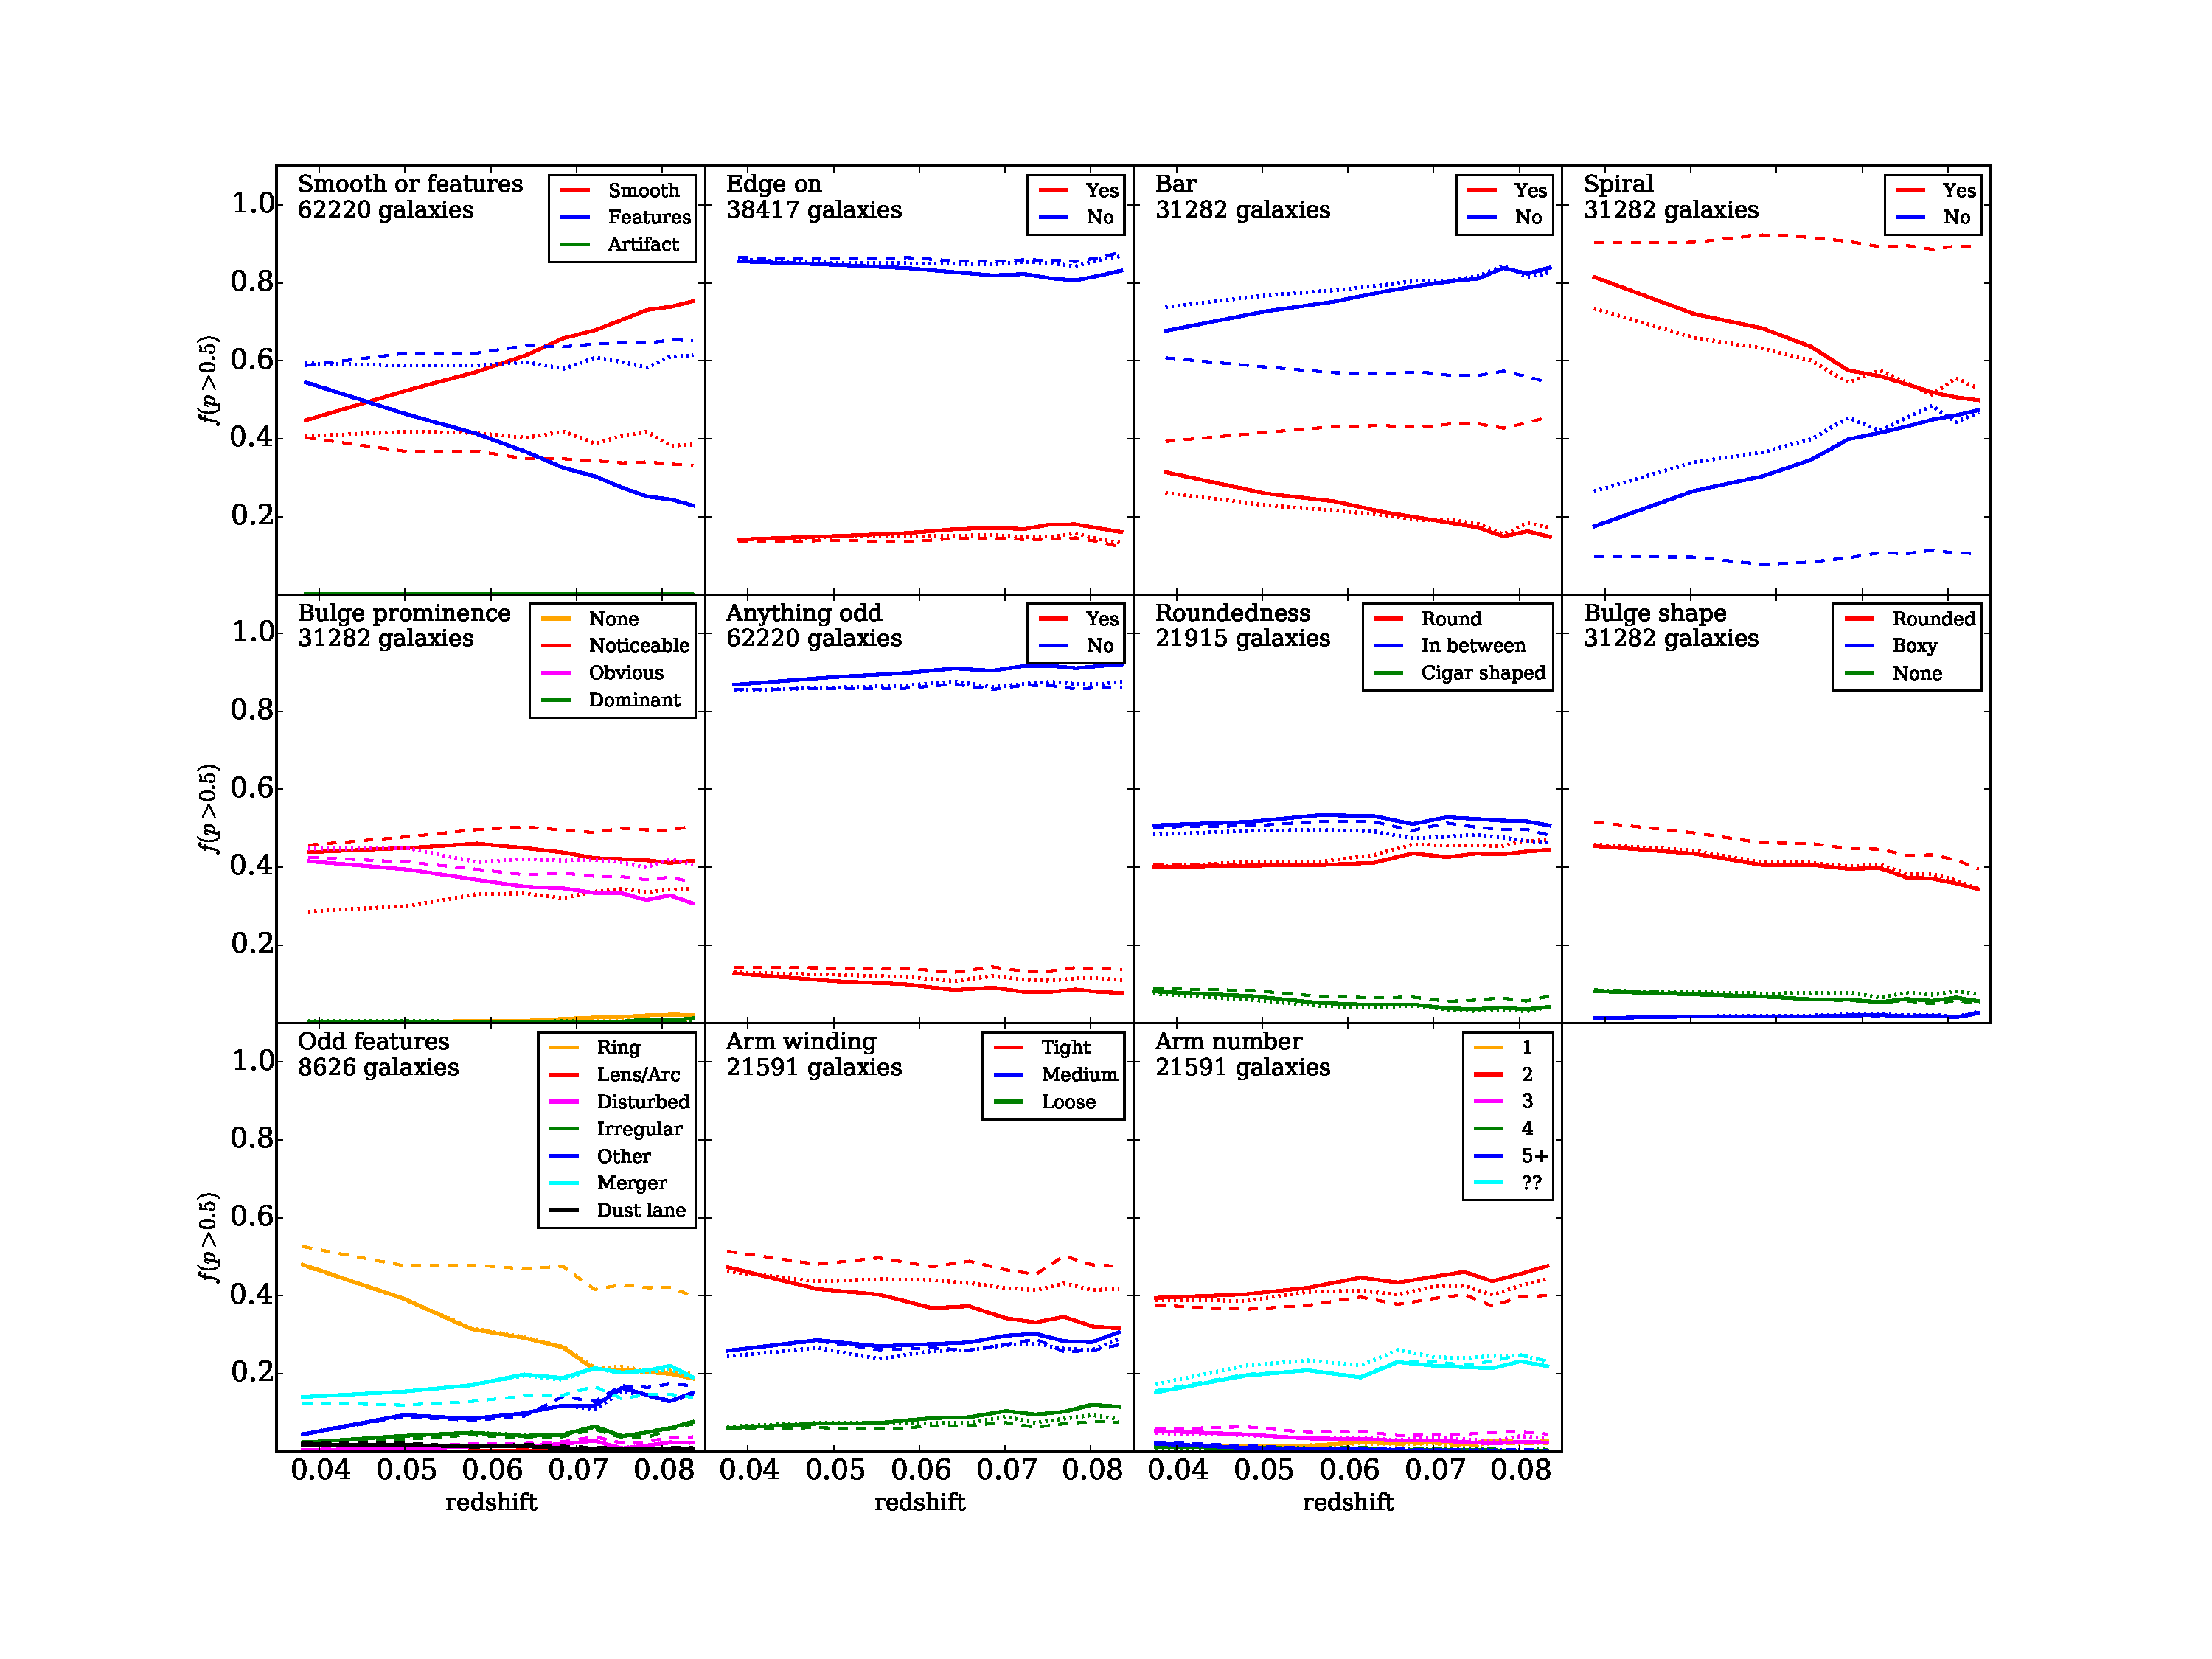
\includegraphics[width=1\textwidth]{Images/Bias/Debiasing/all_thresholds.pdf}

        \caption{Number of galaxies with $p>0.5$ for each of the questions debiased using the method described in section \ref{sec:new_method}. The solid lines indicate the raw vote fractions and the dashed lines indicate the debiased vote fractions. The dotted lines indicate the same fractions using the W13 debiasing method. Each of the samples is composed of galaxies with $p_{\textrm{debiased}}>0.5$ of people having answered that particular question, using the method described in Sec.~\ref{sec:sample_selection_per_question}. The total sample here is composed of galaxies in our \textit{luminosity-limited sample}.}

        \label{fig:all_thresholds}

\end{figure*}

To further compare our raw debiased values with the raw vote fractions and those from W13, we look in to how effectively we match the overall distributions at high and low redshift. Fig.~\ref{fig:all_thresholds} only shows one case in which we choose thresholds at $p>0.5$. However, as described in \ref{sec:new_method}, we aim to match the overall $p$-distributions with redshift. To assess whether our debiasing method is effective at matching the low and high redshift distributions, we plot histograms comparing a low-redshift reference sample with a higher-redshift sample, comparing our debiased values to the raw distributions and those from W13. in Fig.~\ref{fig:all_histograms}.

\rh{Maybe need an RMS of the 'top' end of the distributions to `show' that we're doing better?}

We must also take particular note of the branch of the question tree that we consider. It can be seen from Fig.~\ref{fig:all_thresholds} and Fig.~\ref{fig:all_histograms} that we model the overall fractions of $p_{features}$,$p_{not \, edge-on}$ and $p_{spiral}$ better for the high ends of the distributions, meaning that our samples should be more complete with redshift than if we used the W13 debiasing method. 

\begin{figure*}
		\centering

        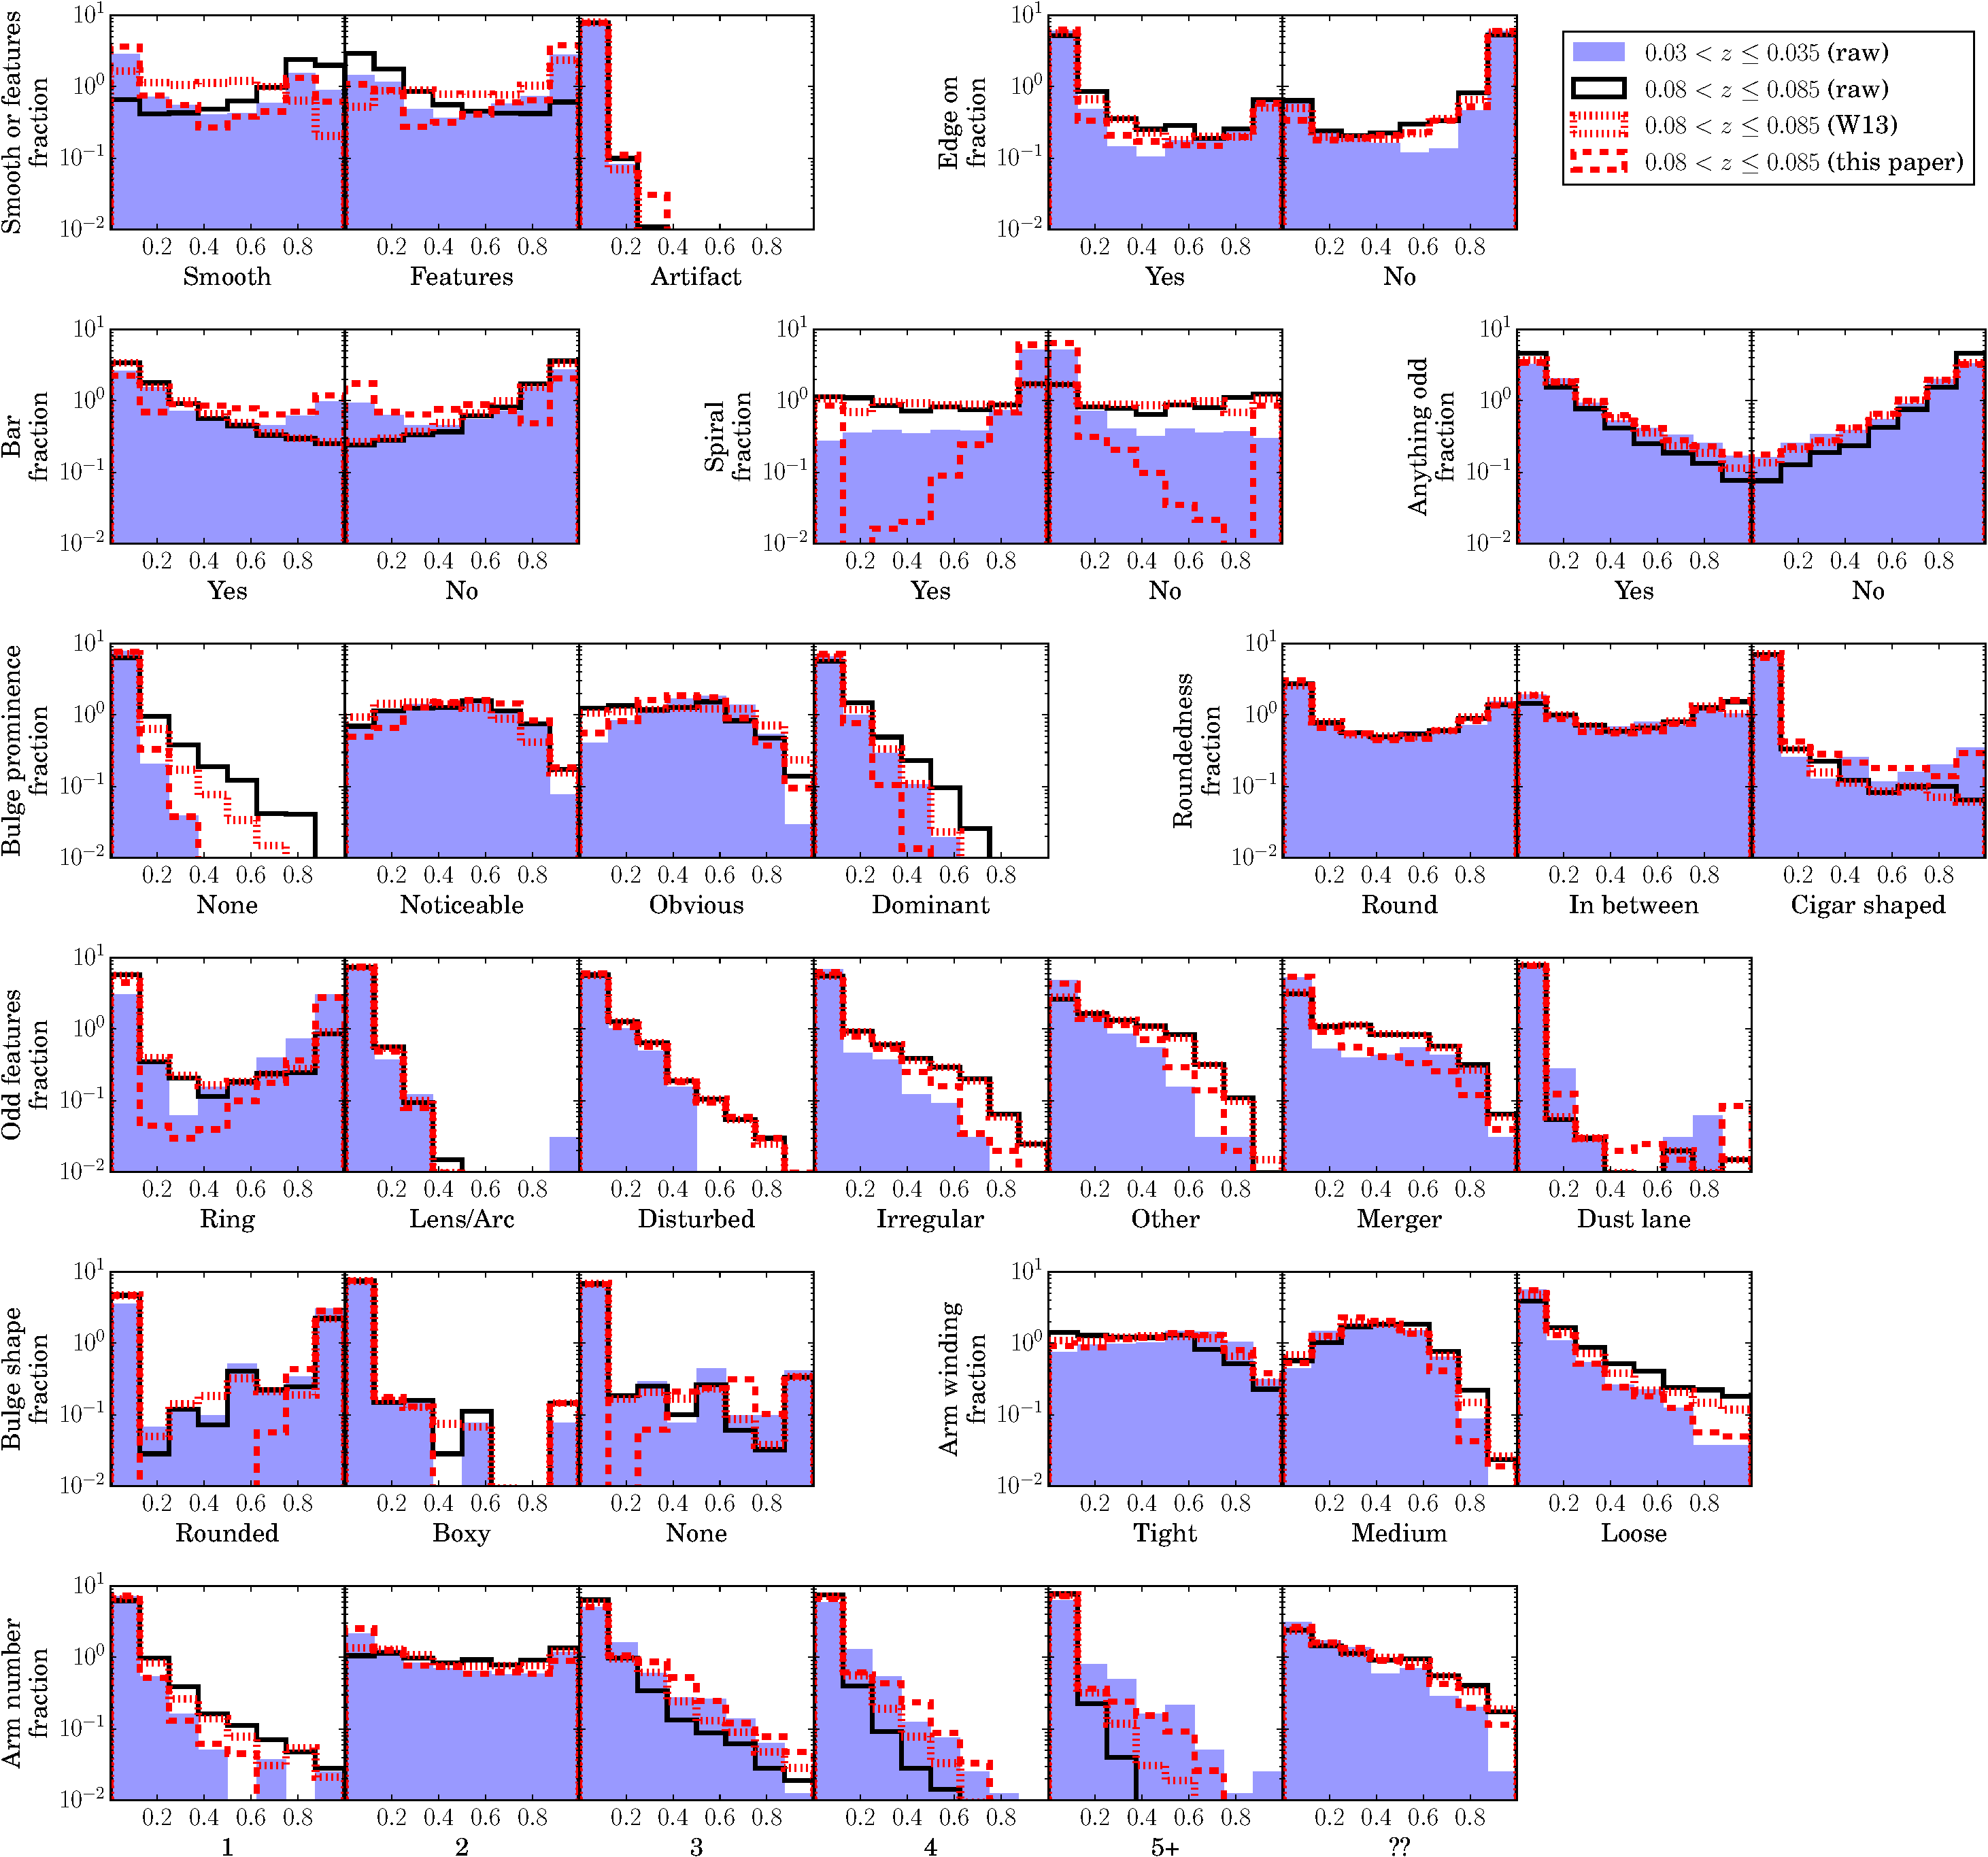
\includegraphics[width=1\textwidth]{Images/Bias/Debiasing/all_histograms.pdf}

        \caption{Vote distribution histograms for each of the answers in the GZ2 question tree. The blue filled histogram shows the distribution for a low redshift $0.03< z \leq 0.035$ sample, which should have minimal redshift-dependent bias. The black solid, red dotted and red dashed histograms show the higher redshift $0.08 < z \leq 0.085$ distribution of the raw, W13 debiased and debiased data from this paper respectively. Both the low and higher redshift distributions are drawn from the \textit{luminosity-limited sample}.}

        \label{fig:all_histograms}

\end{figure*}

%------------------------------------------------------------------------------------
%%%%%%%%%%%%%%%%%%%%%%%%%%%%%%%%%%%%%%%%%%%%%%%%%%%%%%%%%%%%%%%%%%%%%%%%%%%%%%%%%%%%%
%------------------------------------------------------------------------------------
\section{Properties of spiral galaxies with respect to arm number}
\label{sec:results}

We now look in to question 11 of the GZ2 decision tree, which asks users to classify the number of spiral arms that are present in a galaxy. It is well-known that spiral structure can take various forms in local galaxy disks. The main classification scheme to classify the different forms of spiral structure was proposed in \citep{EE_82}, in which spiral structure ranges from `grand design' (containing two long, symmetric spiral arms) to `flocculent' (with multiple fragmented arms). 

Much of the work on comparing spiral galaxies with varying forms of spiral arm structure is related to what types of mechanism could be responsible for different types of spiral structure. In particular, grand design spiral structure can usually be attributed to the presence of a density wave in the galaxy disk \rh{cite}, whereas more flocculent structure is usually asociated with more transient star-formation, enhanced by gravitational and shear effects in the disk. In classical density wave theory, gas is shocked as it enters an overdense environment, causing star-formation. Therefore, modelling star-formation in galaxy disks should give an insight as to whether such a mechanism occurs, as one would expect to see an enhanced star-formation rate (SFR) in two-armed spiral galaxies. However, there is little evidence that this occurs in two-armed spiral galaxies in general \rh{cite}, or in the region of individual spiral arms \rh{cite}. Additionally, an enhancement in the fraction of spirals that exhibit two-armed grand design spiral structure is observed in higher density environments, and with the presence of bars \rh{cite}. However, the interplay between the different processes is still not fully-understood, as strongly barred galaxies, and galaxies in high-density environments can still exhibit spiral structure. Additionally, the type of spiral structure can vary with wavelength, with more grand design spiral structure observed in the infra-red bands that trace the older stellar populations of galaxies. 

Using our debiasing method, we present a robust sample of local galaxies separated by spiral arm number in which to look in to the overall star-formation and environment properties of disk galaxies with respect to the type of spiral structure they exhibit. Here we look at the overall stellar masses, colours and star-formation rates of spiral galaxies, in an attempt to find relationships between overall galaxy demographics and the type of spiral structure they exhibit.

%------------------------------------------------------------------------------------
\subsection{Defining the sample}
\label{sec:defining_the_sample}

We split our sample in to galaxies with 1, 2, 3, 4 or more than 4 spiral arms, using the debiased vote fractions from the method described in Sec.~\ref{sec:new_method}. We define our sample of spiral galaxies  $p_{\textrm{features}} \times p_{\textrm{not edge-on}} \times p_{\textrm{spiral}} > 0.5$. We then assign each of those galaxies to the category with the highest $p$-value when comparing each of the spiral arm answers. To attempt to make the sample as complete as possible, we reassign each of the galaxies which have been classified as `can't tell' by selecingt the sample of galaxies with $N_{spiral} - N_{can't \, tell} > 5$, and reassigning each of those to the category with the next highest value. The fraction of galaxies that make up each of the samples as a function of redshift are shown in figure \ref{fig:arm_number_trend}. 

\begin{figure}
		\centering

        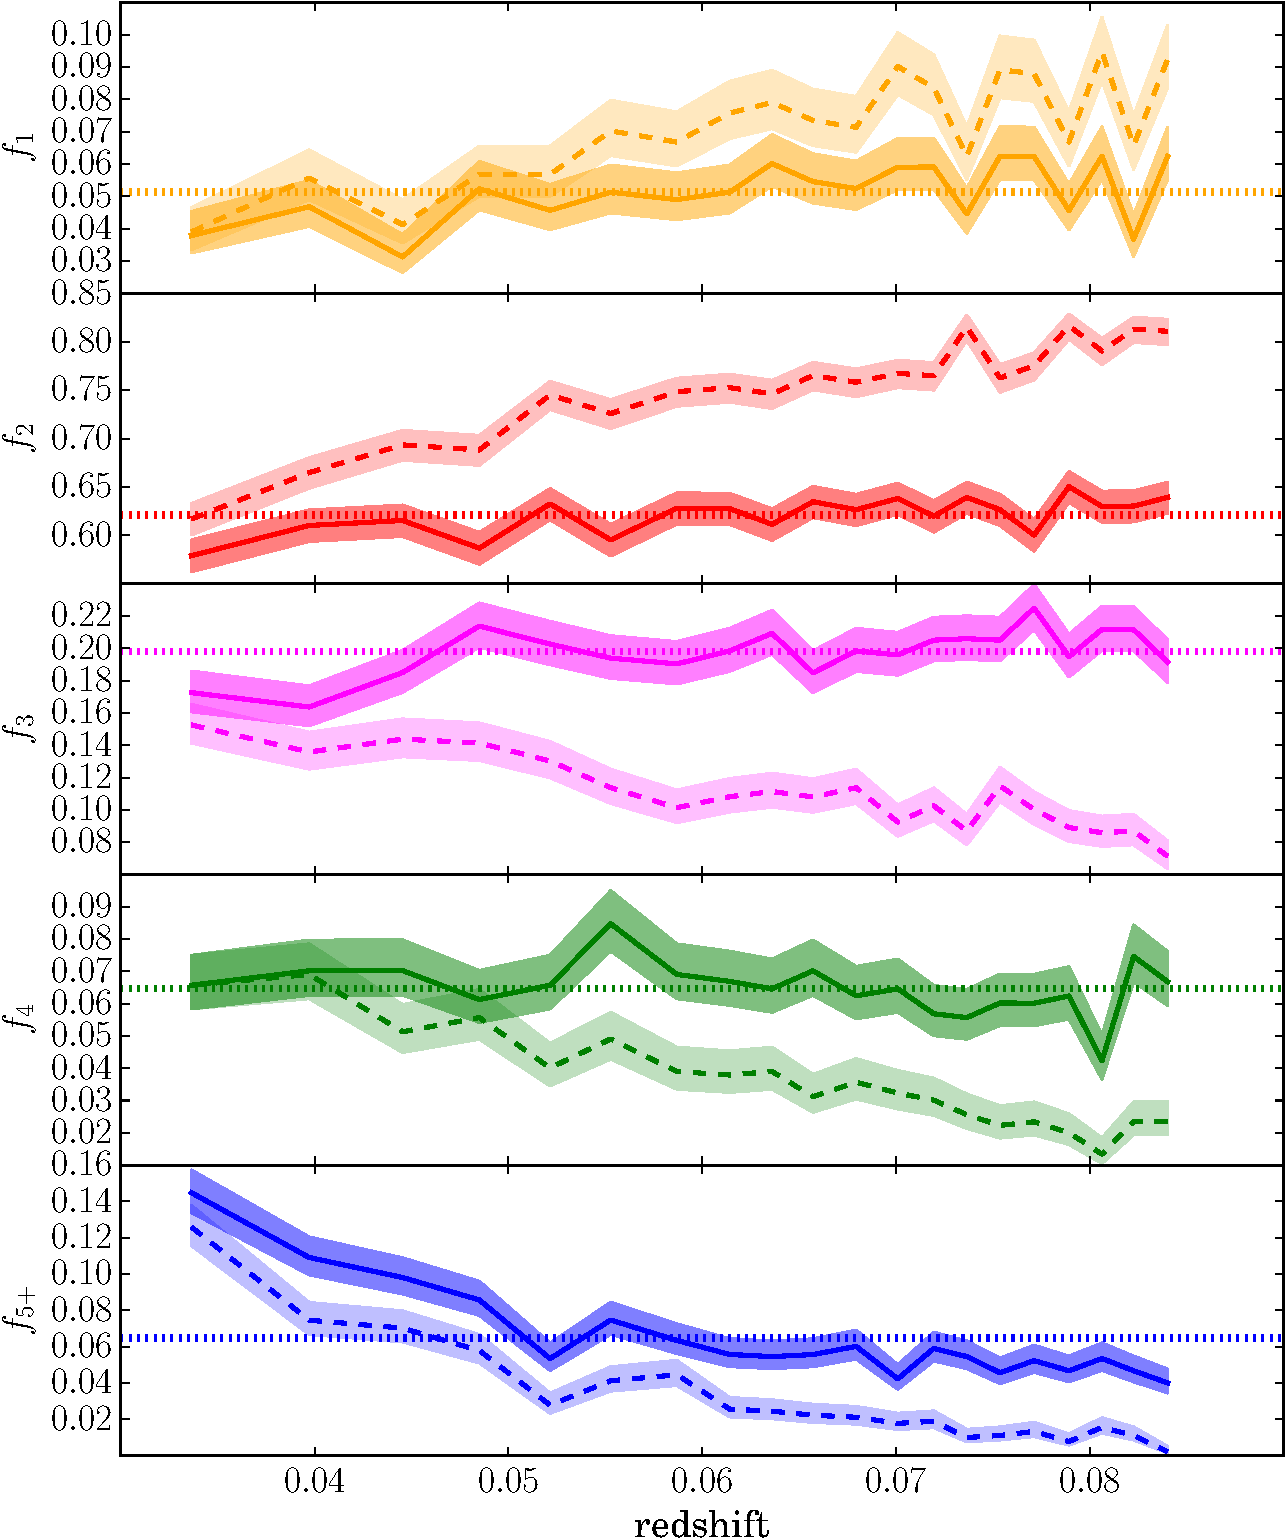
\includegraphics[width=0.5\textwidth]{Images/Results/sample_fractions.pdf}

        \caption{Fraction of galaxies in the \textit{luminosity limited sample} classified as having 1,2,3,4, or more than 4 spiral arms as a function of redshift. The solid line indicates the debiased fractions, and the dashed line indicates the raw vote fractions. Errors are calculated using the method described in \citet{Cameron_11}. The horizontal dotted line shows the mean vote fraction averaged over all of the bins.}

        \label{fig:arm_number_trend}

\end{figure}

%------------------------------------------------------------------------------------
\subsubsection{Comparison of relative sample sizes}

\rh{How big are each of the subsamples, when compared to the literature? This section may need a little more work than originally thought- a lot of the early stuff will deliberately select galaxies in different environments + w or w/o bars, so we may need to do something similar to check our fractions. Maybe use Yang+`s group catalogue, and the GZ bar fractions to define field galaxies and stuff like that to get an estimate of our completeness. This will also have to be compared to the original debiasing to show that we are doing `better' I guess.}

%------------------------------------------------------------------------------------
\subsection{Comparing the overall galaxy populations}

Having defined our samples of spiral galaxies in Sec.~\ref{sec:defining_the_sample}, we now compare the demographics of our different galaxy populations separated by spiral arm number. In particular, we will now look in to the mass, colour and star-formation rates for each of our samples divided by arm number, in order to look in to how the overall stellar populations compare for galaxies with fewer or more spiral arms. The overall sample sizes and properties are listed in table \ref{table:overall_property_table} below.

\begin{table*}

\label{table:overall_property_table}

\begin{tabular}{cccccc}
\hline

$m$                  &   $N_m$ &     $f_m$ & $M_*$ $(\log(M/M_{\odot}))$   & $g-r$         & SFR $(\log(M_{\odot}yr^{-1}))$   \\

\hline
 Luminosity-limited   &   17953 &    1.00    & $10.62\pm 0.25$                      & $0.58\pm 0.10$ & $0.17\pm 0.60$                   \\
 1                    &     922 &    0.05 & $10.63\pm 0.27$                      & $0.58\pm 0.11$ & $0.18\pm 0.70$                   \\
 2                    &   11150 &    0.62 & $10.63\pm 0.24$                      & $0.60\pm 0.10$ & $0.14\pm 0.64$                   \\
 3                    &    3555 &    0.2  & $10.59\pm 0.26$                      & $0.53\pm 0.10$ & $0.28\pm 0.49$                   \\
 4                    &    1162 &    0.06 & $10.60\pm 0.26$                      & $0.53\pm 0.09$ & $0.23\pm 0.47$                   \\
 5+                   &    1164 &    0.06 & $10.65\pm 0.27$                      & $0.54\pm 0.09$ & $0.11\pm 0.52$                   \\
 
\hline
 
 Stellar mass-limited &    9389 &    1.00    & $10.81\pm 0.16$                      & $0.63\pm 0.08$ & $-0.02\pm 0.68$                  \\
 1                    &     495 &    0.05 & $10.83\pm 0.16$                      & $0.65\pm 0.09$ & $-0.07\pm 0.79$                  \\
 2                    &    6039 &    0.64 & $10.81\pm 0.15$                      & $0.65\pm 0.07$ & $-0.07\pm 0.71$                  \\
 3                    &    1655 &    0.18 & $10.82\pm 0.16$                      & $0.59\pm 0.07$ & $0.15\pm 0.60$                   \\
 4                    &     564 &    0.06 & $10.82\pm 0.16$                      & $0.58\pm 0.07$ & $0.12\pm 0.56$                   \\
 5+                   &     636 &    0.07 & $10.85\pm 0.18$                      & $0.58\pm 0.07$ & $-0.04\pm 0.57$                  \\

\hline

\end{tabular}

\caption{Overall properties of galaxy populations with different numbers of spiral arms. The number of galxies with 1,2,3,4 and more than 4 arms are shown for both the \textit{luminosity-limited} and \textit{stellar mass-limited} spiral samples. Mean stellar masses, colours and star-formation rates are shown for each of the populations, with $1\sigma$ standard deviations.}

\end{table*}

%------------------------------------------------------------------------------------
\subsubsection{Stellar mass}

\begin{figure}
		\centering

        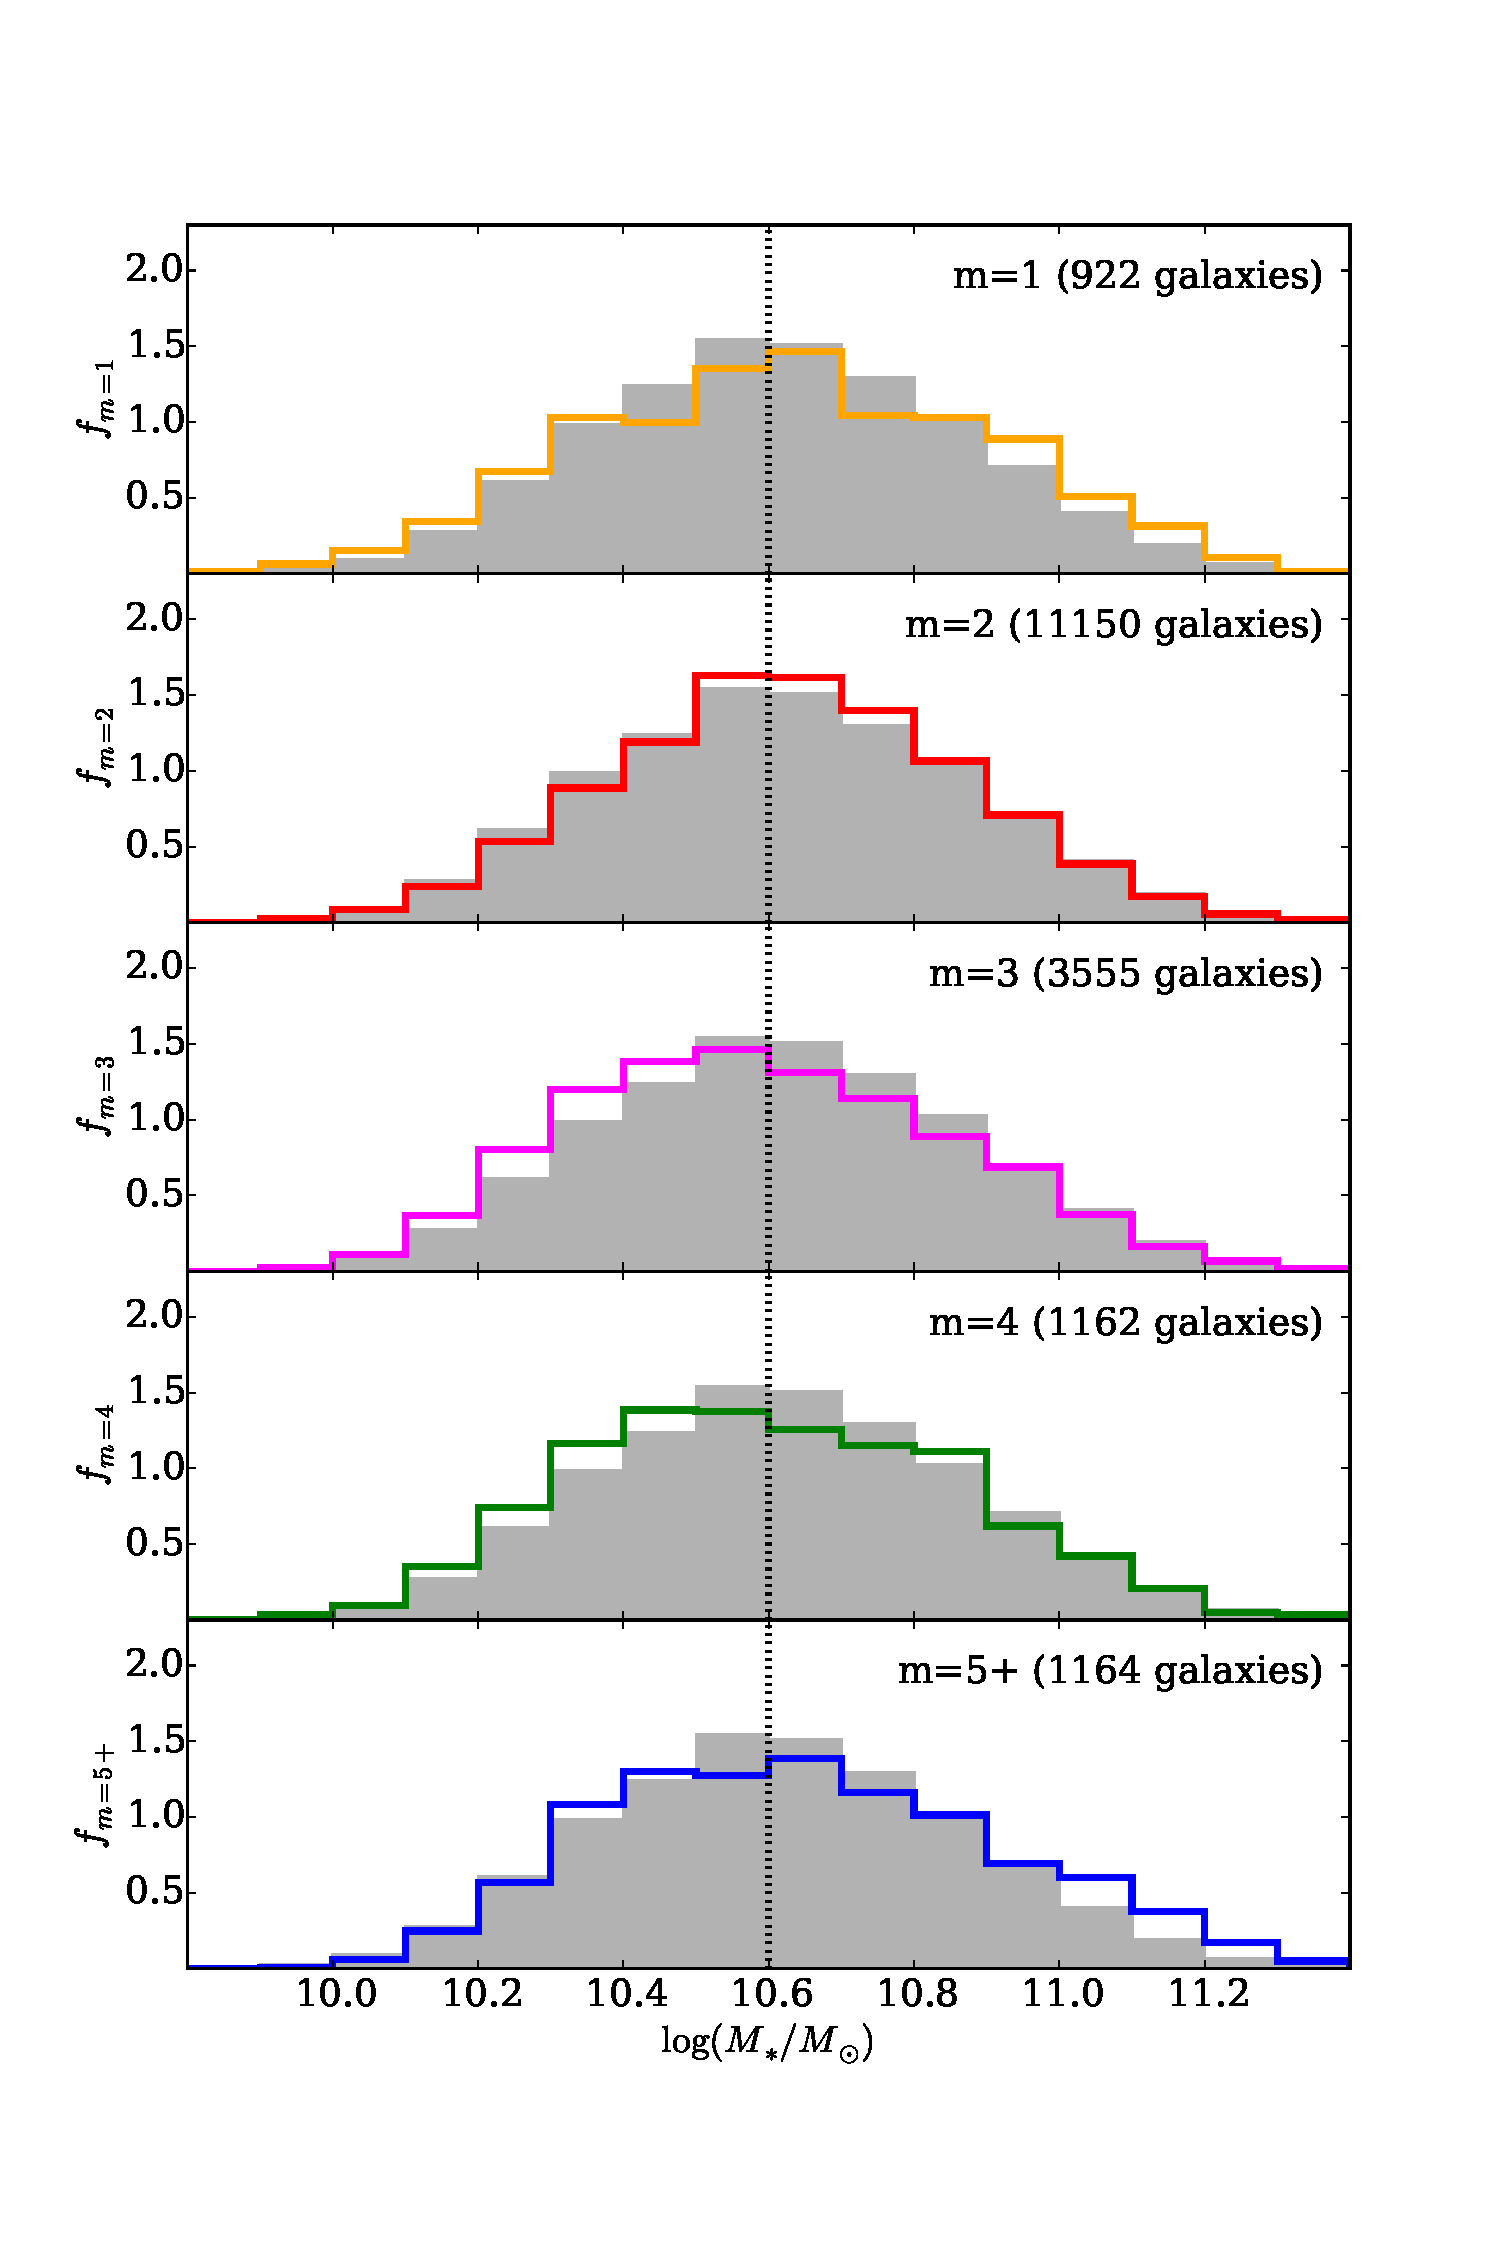
\includegraphics[width=0.5\textwidth]{Images/Results/mass_histograms.pdf}

        \caption{Distributions of the stellar masses for each of the \emph{arm number samples}. The black dotted line shows the $M_*$ values above which the \textit{luminosity-limited sample is complete}. The filled grey histograms show the same distibution for the overall \textit{spiral sample} (taken from the \textit{luminosity-limited sample}).}

        \label{fig:mass_histograms}

\end{figure}

%------------------------------------------------------------------------------------
\subsubsection{Galaxy colours}
%------------------------------------------------------------------------------------

\subsubsection{Local environment}

%------------------------------------------------------------------------------------

\subsubsection{Star formation rate}
\label{sec:sfr}

\begin{figure}
		\centering

        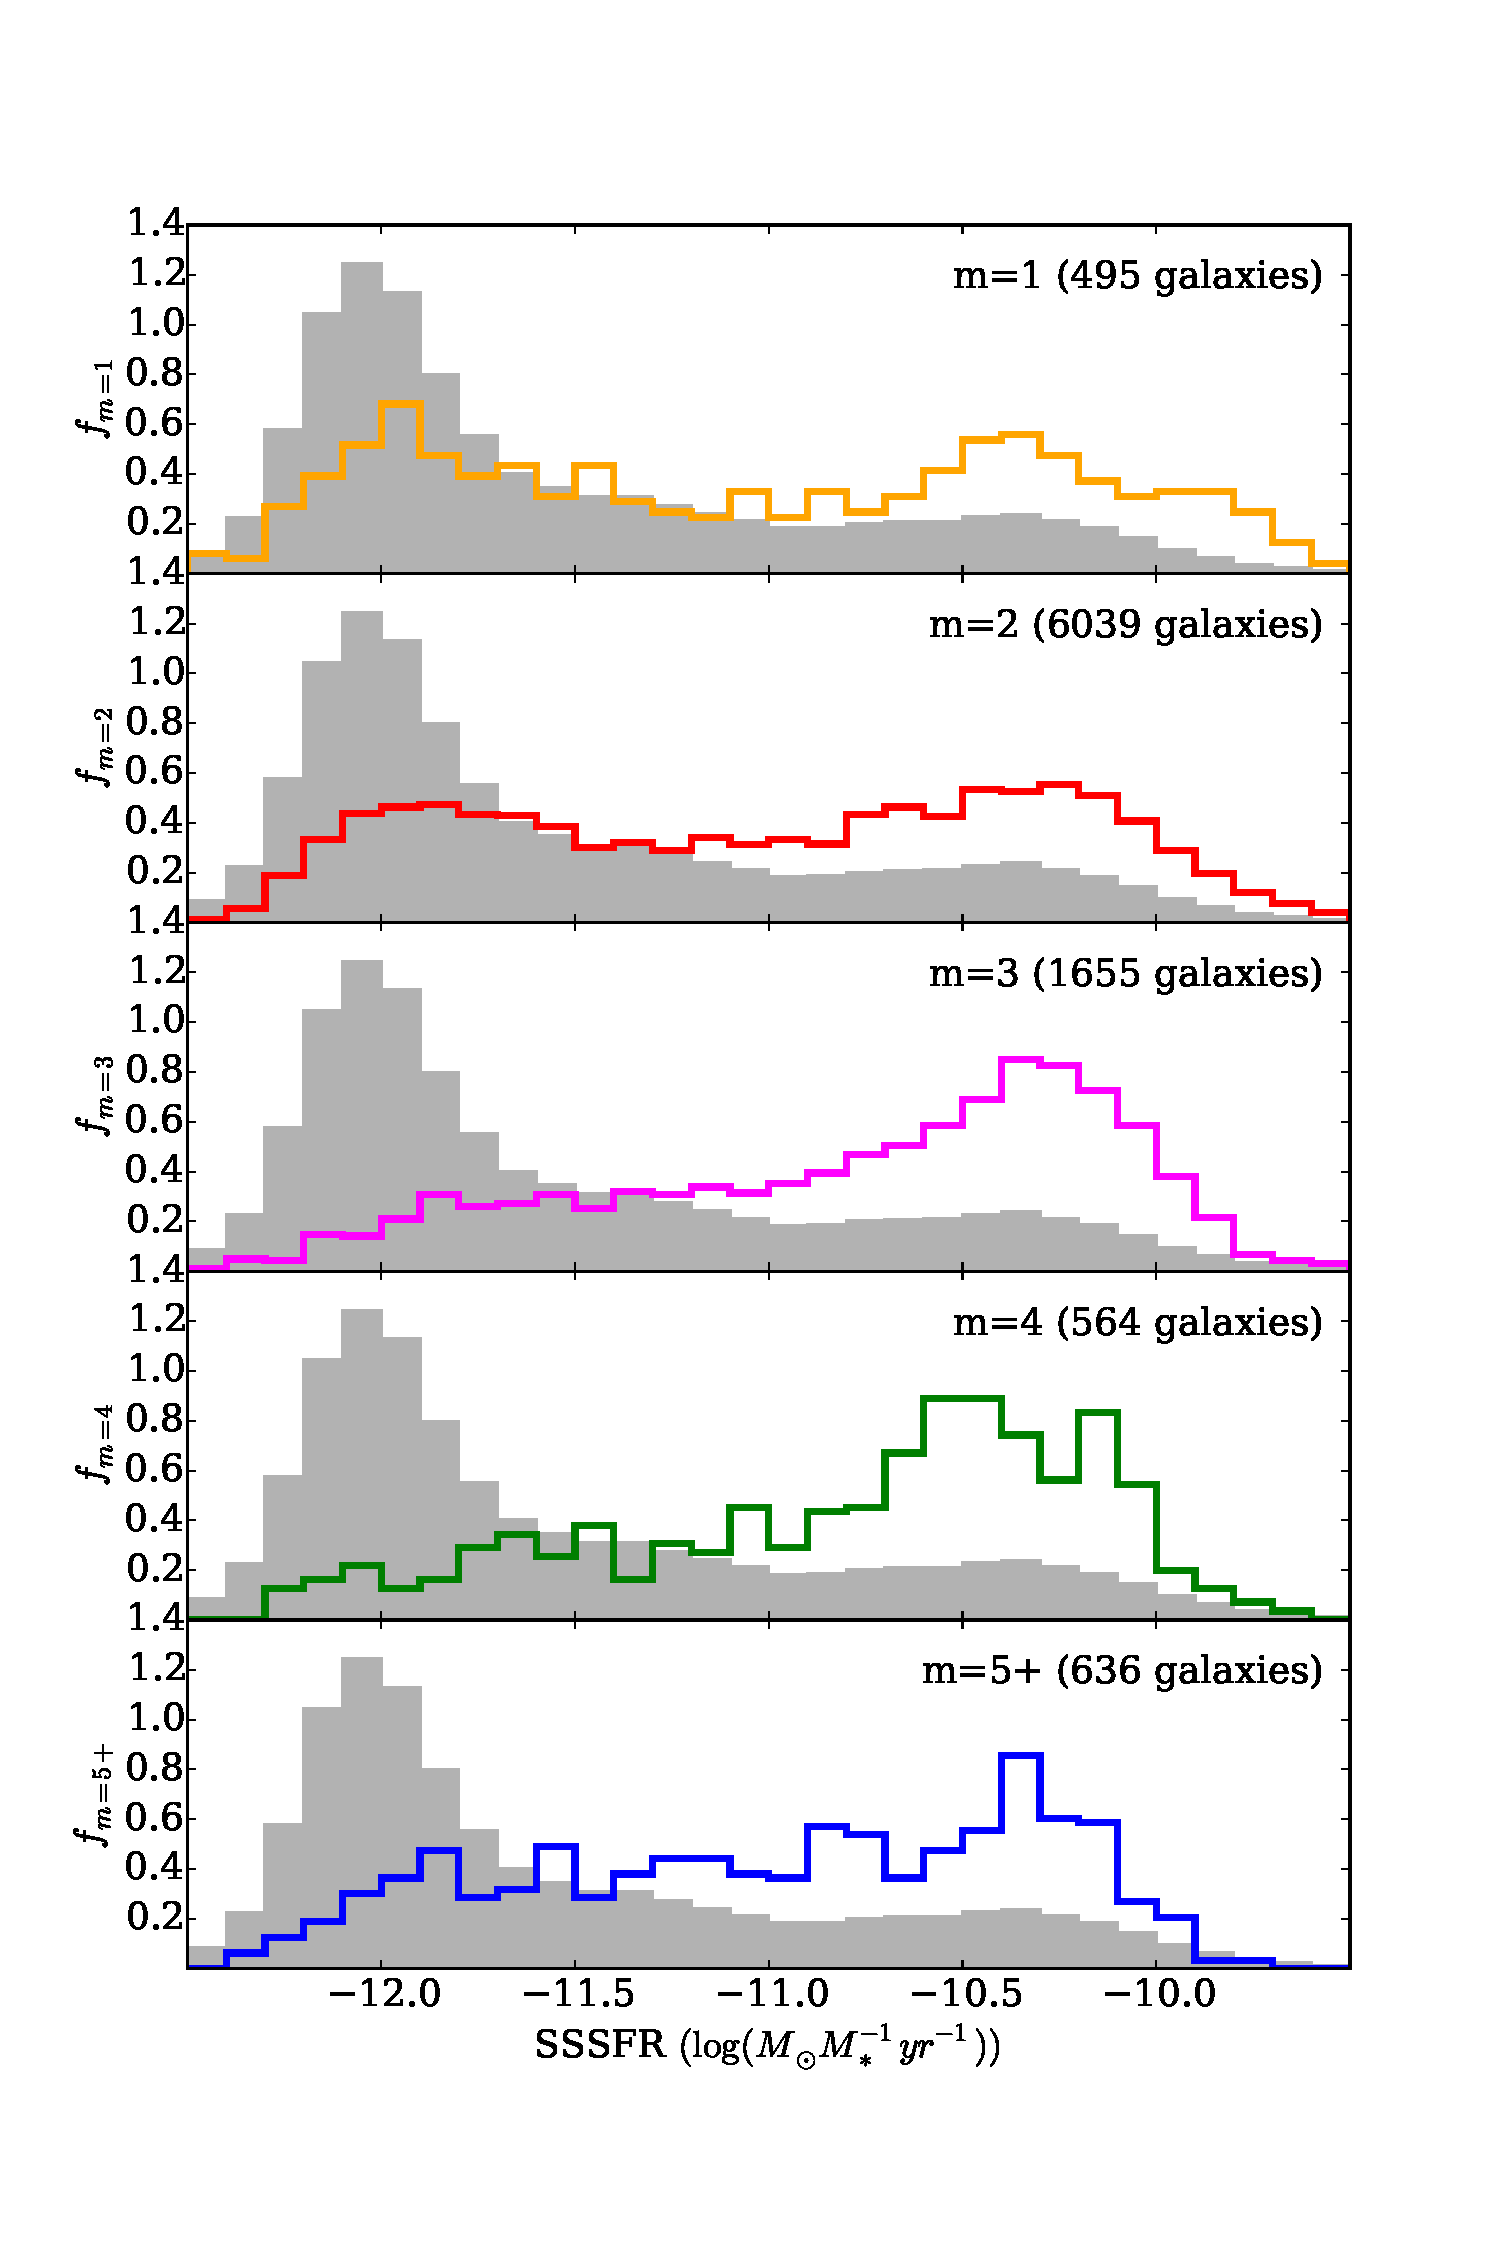
\includegraphics[width=0.5\textwidth]{Images/Results/sfr_histograms.pdf}

        \caption{Distributions of the SFRs of each of the \emph{arm number samples}. Each of the samples is defined in in the way described in Sec.~\ref{sec:defining_the_sample}, and taken from the \emph{stellar mass-limited sample}. The grey underplotted histograms show the equivalent distribution for the total \textit{stellar mass-limited sample}.}

        \label{fig:sfr_histograms}

\end{figure}
%------------------------------------------------------------------------------------
%%%%%%%%%%%%%%%%%%%%%%%%%%%%%%%%%%%%%%%%%%%%%%%%%%%%%%%%%%%%%%%%%%%%%%%%%%%%%%%%%%%%%
%------------------------------------------------------------------------------------
\section{Conclusions}
\label{sec:conclusions}

An examination of the properties of spiral galaxies with respect to their disk structure is presented using statistical morphological data from Galaxy Zoo. We show that employing a new debiasing procedure allows us to compare the properties of a spectroscopically complete sample of XX galaxies, of which XX can be classified as spirals and compared in terms of spiral arm number. Using this new debiasing method, clear differences in the overall properties of spiral galaxies are observed. By defining a stellar mass limited sample of spiral galaxies, it is seen that galaxies with greater numbers of spiral arms have higher stellar masses \rh{(Numbers?)}. A clear trend is also observed with respect to galaxy colour, with 4 and more than 4 armed spiral galaxies being much bluer in the $g-r$ colour band. The most stark contrast is observed when comparing the 2 armed spiral galaxy population with the more than 4 armed spiral galaxy population- we observe that for a given stellar mass, more than 4 armed spiral galaxies are $XX \pm XX$ bluer in $g-r$ than 2 armed spiral galaxies. However, there is no significant difference observed in the star formation rates of galaxies with different numbers of spiral arms. This suggests  that the $g-r$ colour differences are not attributable to more recent star formation in more than 4 armed spiral galaxies, and may therefore be due to 2 armed spiral galaxies having an older overall stellar population, or containing more dust.

%------------------------------------------------------------------------------------
%%%%%%%%%%%%%%%%%%%%%%%%%%%%%%%%%%%%%%%%%%%%%%%%%%%%%%%%%%%%%%%%%%%%%%%%%%%%%%%%%%%%%
%------------------------------------------------------------------------------------

\section{Acknowledgements}

The data in this paper are the result of the efforts of the Galaxy Zoo 2 volunteers, without whom none of this work would be possible. Their efforts are individually acknowledged at authors.galaxyzoo.org.

\bibliographystyle{mn2e}
\bibliography{jun15}


\appendix
\section{Examples of galaxy images}

We now present some example galaxy images as a function of redshift. We define two samples- one with $0.5< p \leq 0.6$ for each arm number question, and one with $p > 0.8$ in Fig. ~\ref{fig:image_panel},and a more secure sample of galaxies with $p > 0.8$ in Fig.~\ref{fig:image_panel_secure}. It is immediately apparent that the raw vote fractions do change as a function of redshift, with the overall $p_{raw}$ vote fraction being lower in the higher redshift sample for the 4 and more than 4 armed spiral galaxy categories. Correspondingly, the overall vote fractions for the categories with fewer spiral arms (the 1 or 2 spiral arm categories) increase with redshift. \rh{What point are we making here???}

\begin{figure*}
		\centering

        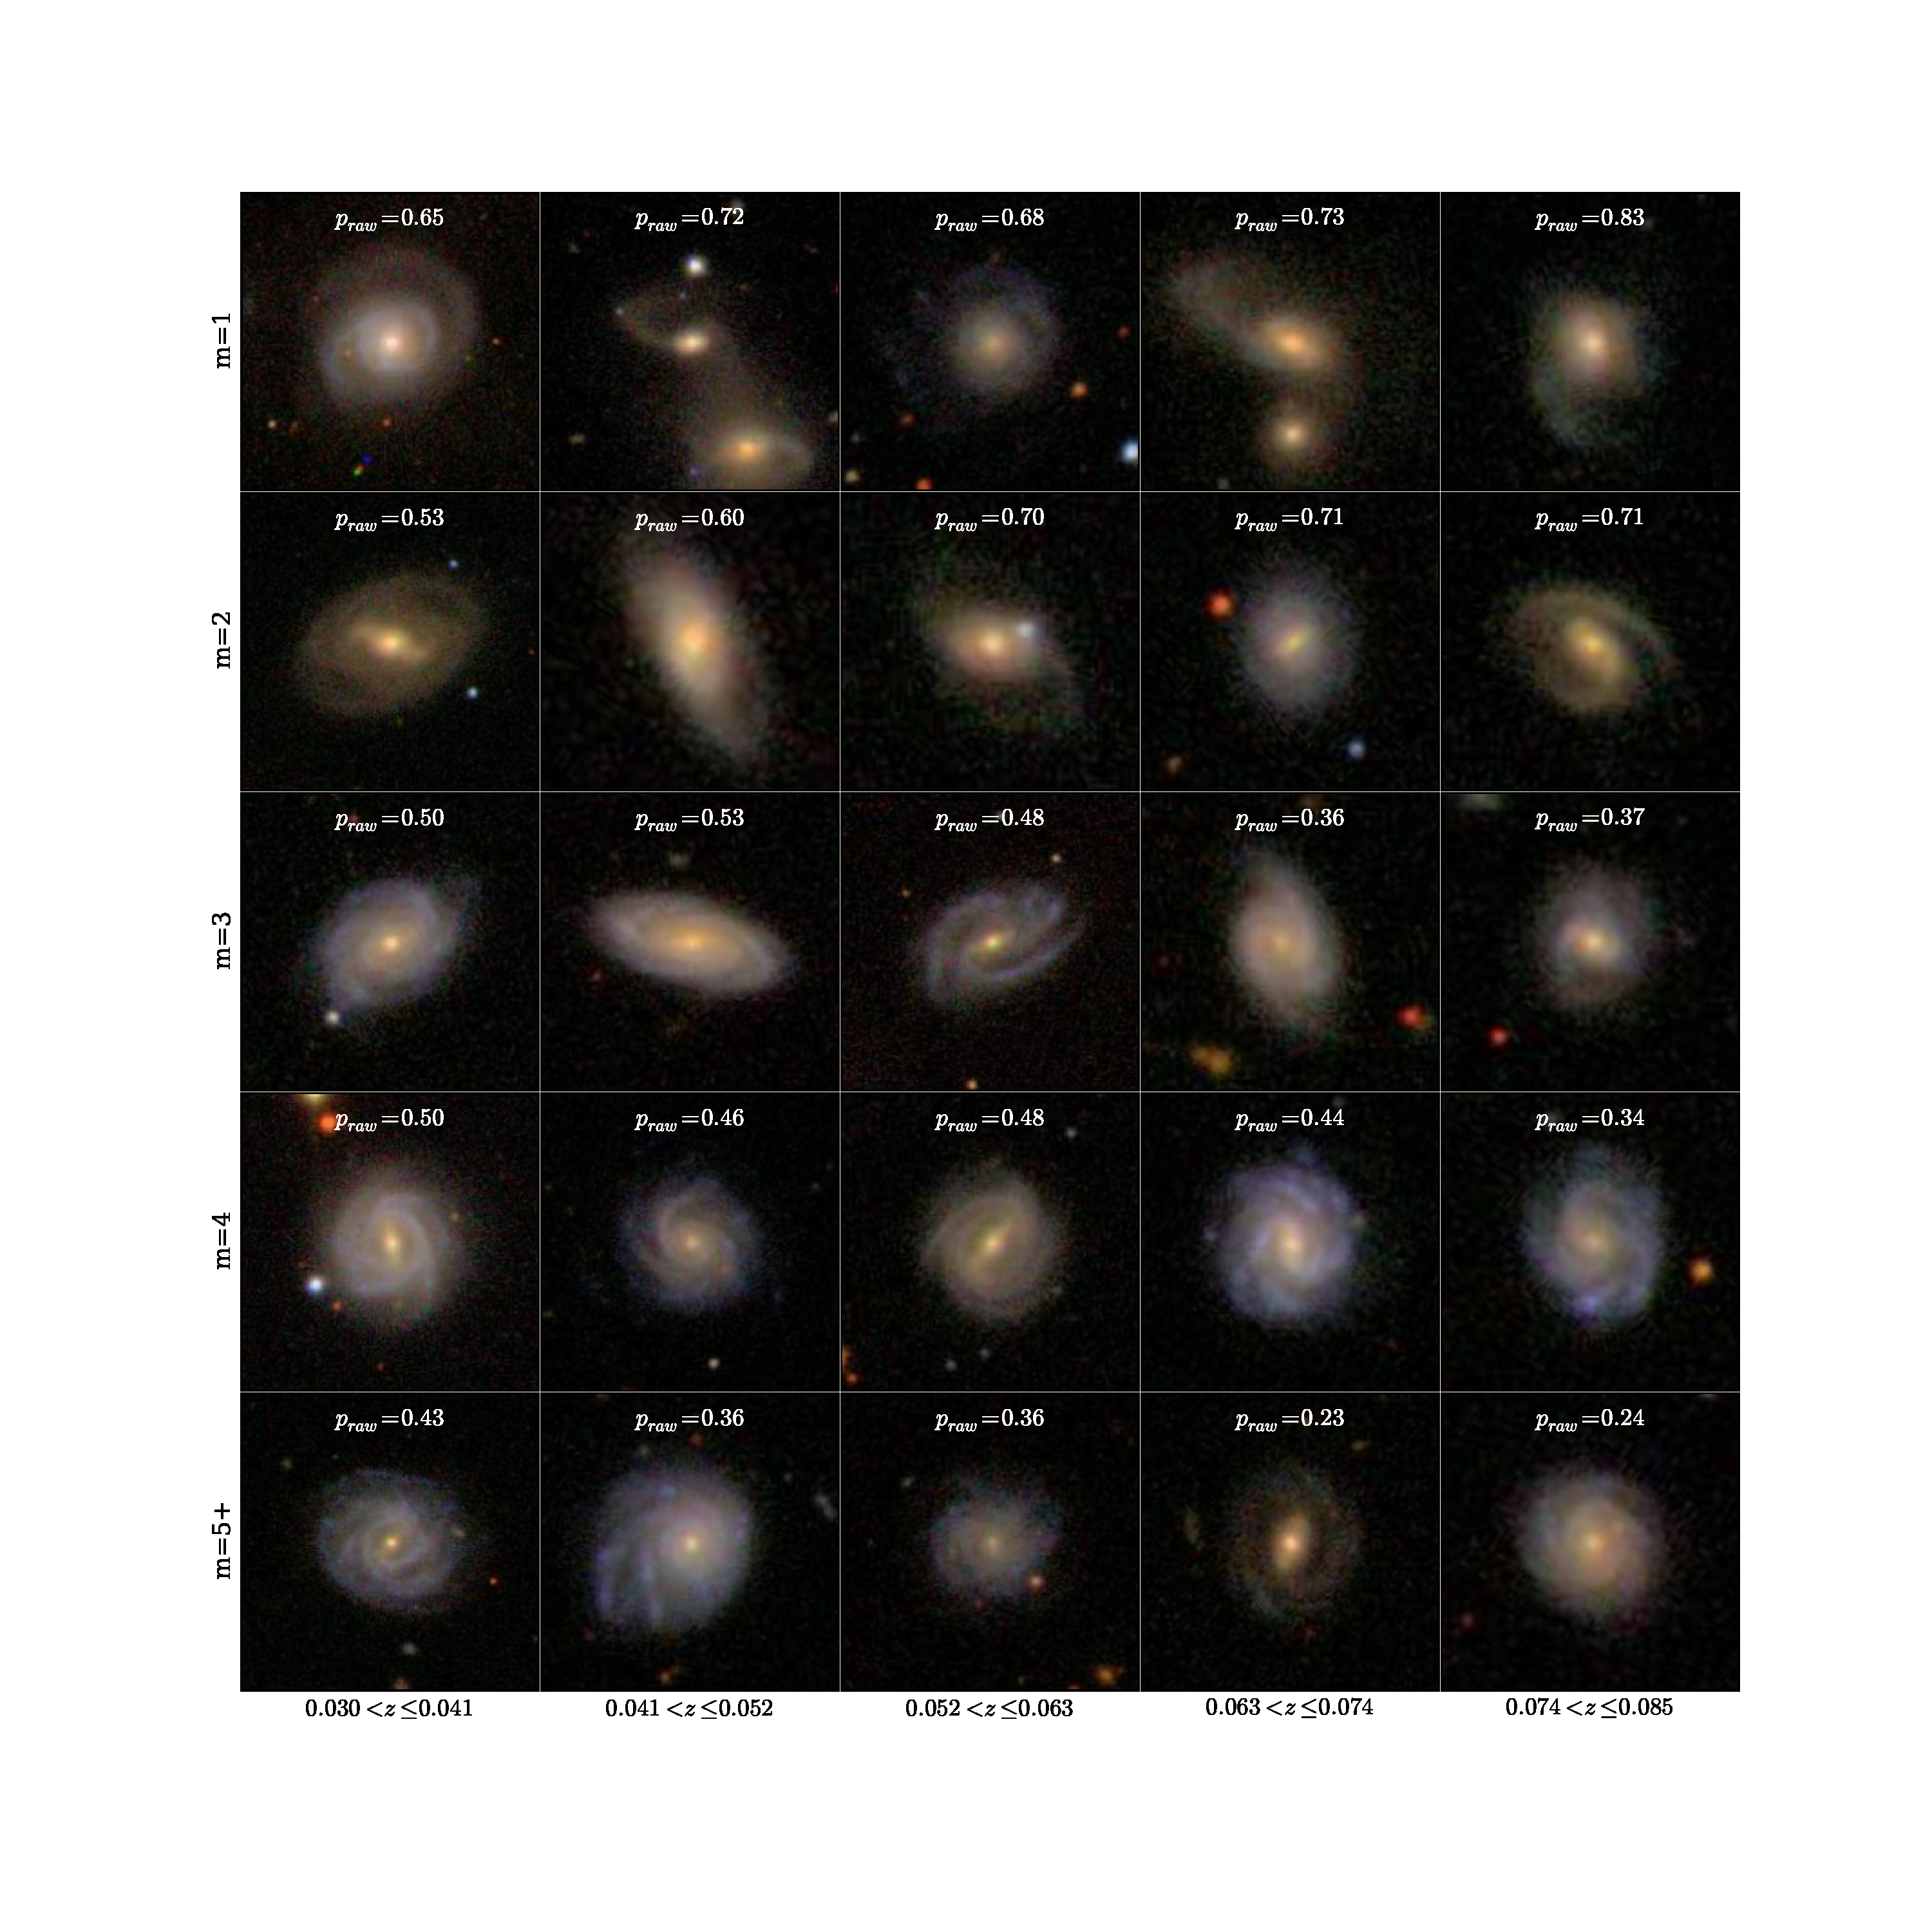
\includegraphics[width=1\textwidth]{Images/Results/image_page_p0506_m106110.pdf}

        \caption{Galaxies classified as 1,2,3,4 or more than 4 armed in different redshift ($z$) bins. Each of the galaxies is within a stellar mass range of $10.6 \leq \log(M/M_{\odot}) < 11.0$. The modal $p_m$ value (where $m$ is the spiral arm number) is within the range $0.5 \leq p_m < 0.6$.}

        \label{fig:image_panel}

\end{figure*}

\begin{figure*}
		\centering

        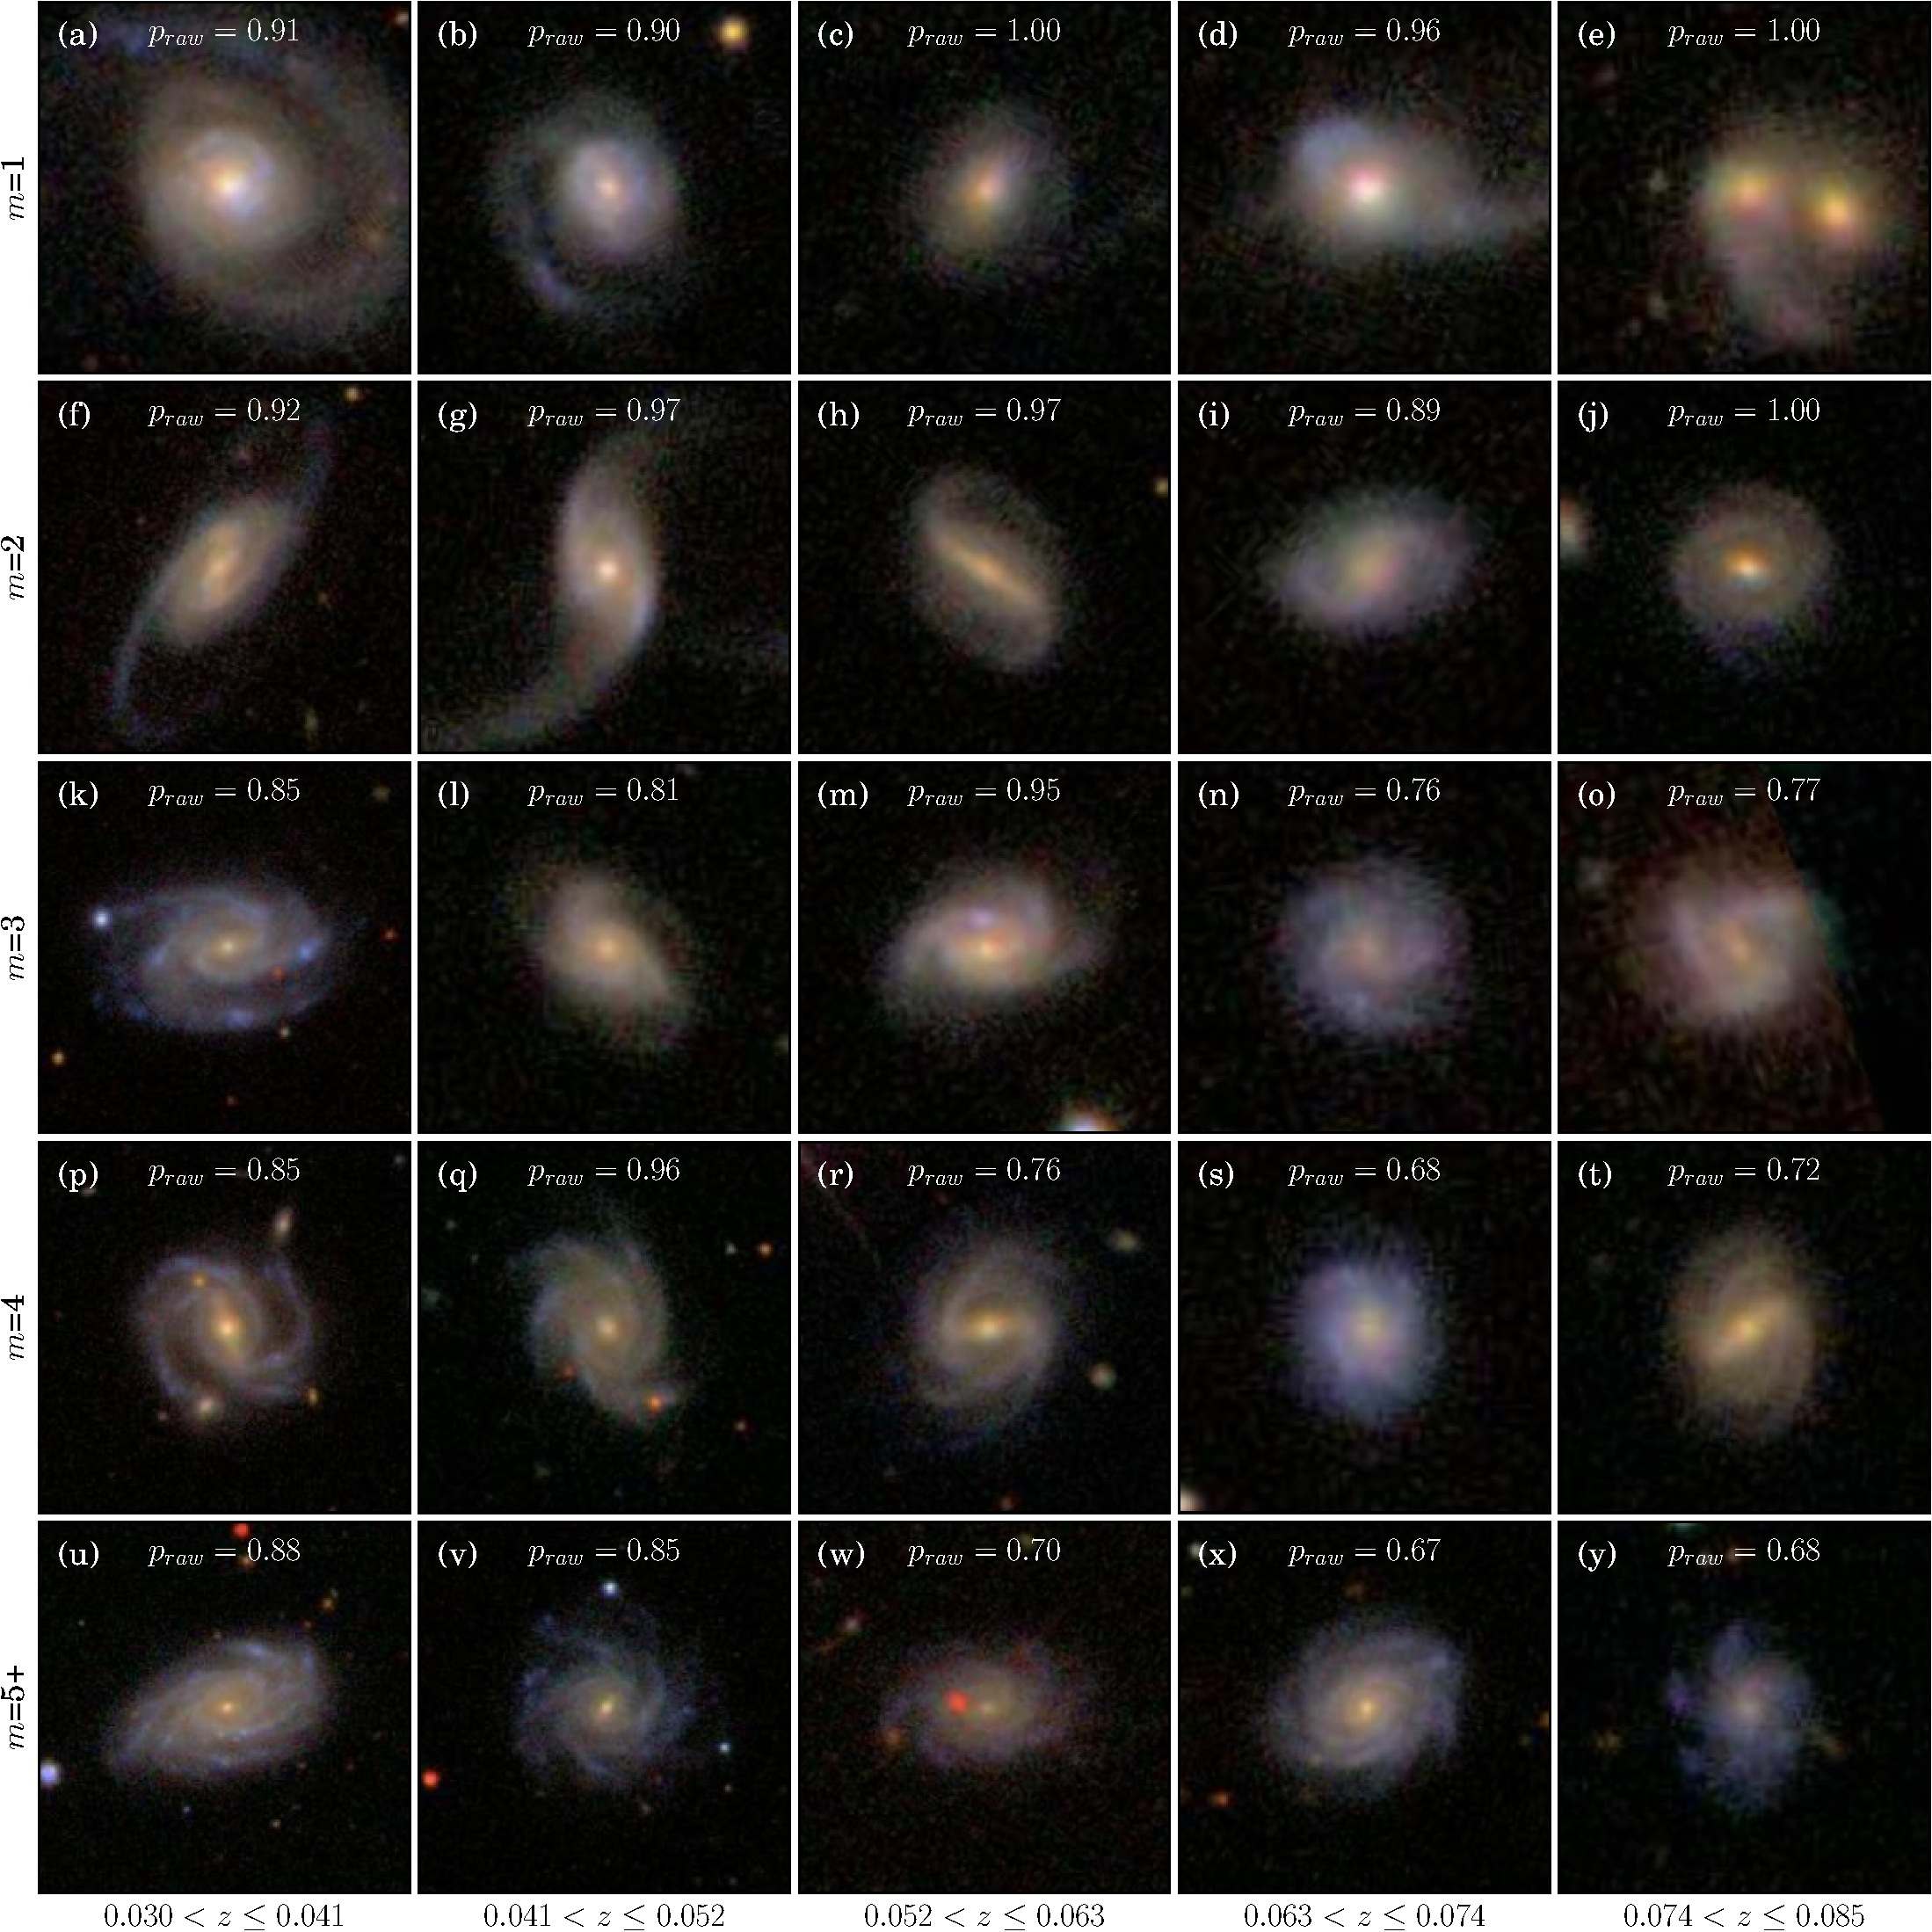
\includegraphics[width=1\textwidth]{Images/Results/image_page_p0810_m106110.pdf}

        \caption{Galaxies classified as 1,2,3,4 or more than 4 armed in different redshift ($z$) bins. Each of the galaxies is within a stellar mass range of $10.6 \leq \log(M/M_{\odot}) < 11.0$. Each of the galaxies has a modal $p$-value of $p_m > 0.8$.}

        \label{fig:image_panel_secure}

\end{figure*}



\end{document}
